% =============================================================================
% CRT-Royale MSL -- Projektdokumentation
% Software-Projekt, SS 2026
% Hochschule Karlsruhe (HKA)
% =============================================================================
\documentclass[11pt, a4paper]{article}

% --- Pakete ---
\usepackage[ngerman]{babel}
\usepackage[utf8]{inputenc}
\usepackage[T1]{fontenc}
\usepackage{lmodern}
\usepackage[left=2.5cm, right=2.5cm, top=2.5cm, bottom=2.5cm]{geometry}
\usepackage{graphicx}
\usepackage[table]{xcolor}
\usepackage{hyperref}
\usepackage{enumitem}
\usepackage{tabularx}
\usepackage{booktabs}
\usepackage{tikz}
\usepackage{float}
\usepackage{fancyhdr}
\usepackage{titlesec}
\usepackage{parskip}
\usepackage{listings}
\usepackage{tcolorbox}
\usepackage{amsmath}
\usepackage{amssymb}
\usepackage{tocloft}
\usepackage{colortbl}
\usepackage[justification=centering]{caption}
\usepackage{etoolbox}

% --- Tabellen-Styling: alternierende Zeilen ---
\newcommand{\tableheadercolor}{\rowcolor{hkared}}
\newcommand{\thw}[1]{\color{white}\textbf{#1}}  % table header white
\setlength{\aboverulesep}{0pt}
\setlength{\belowrulesep}{0pt}
\setlength{\extrarowheight}{3pt}
\renewcommand\tabularxcolumn[1]{m{#1}}

\usetikzlibrary{arrows.meta, positioning, calc, shapes.geometric, fit}

% --- Farben (HKA Corporate) ---
\definecolor{hkared}{RGB}{198, 42, 18}
\definecolor{hkagray}{RGB}{100, 100, 100}
\definecolor{codebg}{RGB}{245, 245, 245}
\definecolor{codeframe}{RGB}{200, 200, 200}
\definecolor{keywordblue}{RGB}{0, 0, 180}
\definecolor{commentgreen}{RGB}{0, 128, 0}
\definecolor{stringred}{RGB}{163, 21, 21}

% --- Hyperref Setup ---
\hypersetup{
    colorlinks=true,
    linkcolor=.,
    urlcolor=hkared,
    citecolor=hkared
}

% --- Code Listings ---
\lstdefinelanguage{Metal}{
    morekeywords={kernel, void, float, float2, float3, float4, half, half4,
        uint, uint2, int, bool, struct, namespace, constant, device,
        texture2d, sampler, thread, threadgroup, access, read, write,
        if, else, return, for, using},
    sensitive=true,
    morecomment=[l]{//},
    morecomment=[s]{/*}{*/},
    morestring=[b]",
}

\lstset{
    basicstyle=\ttfamily\small,
    backgroundcolor=\color{codebg},
    frame=single,
    rulecolor=\color{codeframe},
    keywordstyle=\color{keywordblue}\bfseries,
    commentstyle=\color{commentgreen}\itshape,
    stringstyle=\color{stringred},
    numbers=left,
    numberstyle=\tiny\color{hkagray},
    numbersep=8pt,
    breaklines=true,
    tabsize=4,
    showstringspaces=false,
    captionpos=b,
    xleftmargin=1.5em,
    framexleftmargin=1.5em,
}

% --- Section Styling (Text) ---
% Große Kapitel: schwarz, größer
\titleformat{\section}{\Large\bfseries}{\thesection}{1em}{}
% Unterkapitel: rot
\titleformat{\subsection}{\normalsize\bfseries\color{hkared}}{\thesubsection}{1em}{}
\titleformat{\subsubsection}{\normalsize\itshape\color{hkared}}{\thesubsubsection}{1em}{}
\titlespacing*{\section}{0pt}{1.5em}{0.6em}
\titlespacing*{\subsection}{0pt}{0.8em}{0.3em}
\titlespacing*{\subsubsection}{0pt}{0.6em}{0.2em}

% --- Inhaltsverzeichnis Styling ---
% Große Kapitel: Text schwarz bold, Seitenzahl rot bold
\renewcommand{\cftsecfont}{\bfseries\color{black}}
\renewcommand{\cftsecpagefont}{\bfseries\color{hkared}}
\renewcommand{\cftsecleader}{\color{hkared}\cftdotfill{\cftsecdotsep}}
\renewcommand{\cftsecdotsep}{\cftdotsep}
% Unterkapitel: Nummer+Text rot, Punkte rot, Seitenzahl schwarz
\renewcommand{\cftsubsecfont}{\color{hkared}}
\renewcommand{\cftsubsecpagefont}{\color{black}}
\renewcommand{\cftsubsecleader}{\color{hkared}\cftdotfill{\cftsubsecdotsep}}
\renewcommand{\cftsubsubsecfont}{\color{hkared}}
\renewcommand{\cftsubsubsecpagefont}{\color{black}}
\renewcommand{\cftsubsubsecleader}{\color{hkared}\cftdotfill{\cftsubsubsecdotsep}}
% Abstände: Luft vor Kapitel, Untereinträge eng
\setlength{\cftbeforesecskip}{0.8em}
\setlength{\cftbeforesubsecskip}{0.15em}
\setlength{\cftbeforesubsubsecskip}{0.1em}
% Abstand NACH Kapitel-Zeile (vor erstem Untereintrag)
\renewcommand{\cftsecafterpnum}{\vskip 0.3em}
% Abstand nach "Inhaltsverzeichnis"-Überschrift
\setlength{\cftaftertoctitleskip}{1cm}

% --- Header/Footer ---
\pagestyle{fancy}
\fancyhf{}
\fancyhead[L]{\small\color{hkagray}CRT-Royale {[MSL]} -- Projektdokumentation}
\fancyhead[R]{\small\color{hkagray}Software-Projekt SS~2026}
\fancyfoot[C]{\small\color{hkagray}\thepage}
\renewcommand{\headrulewidth}{0.4pt}

% =============================================================================
\begin{document}

% --- Titelseite ---
\begin{titlepage}
    \centering
    
\includegraphics[width=0.35\textwidth]{HKA.jpg}

    {\normalsize\color{hkagray} University of Applied Sciences}\\[0.125cm]
    {\small\color{hkagray} Fakult\"at f\"ur Informatik und Wirtschaftsinformatik}

    \vspace{.5cm}
    {\color{hkared}\rule{\textwidth}{1.5pt}}

    \vspace{1.5cm}
    {\fontsize{24}{30}\selectfont\bfseries\color{hkared} CRT-Royale {[MSL]}}\\[1cm]
    {\Large Portierung von CRT-Royale in die Metal Shading Language \newline sowie Implementierung in RetroVisor}\\[1cm]
    {\LARGE\bfseries Projektdokumentation}

    \vspace{1cm}
    {\large Software-Projekt}\\
    {\large Sommersemester 2026}

    \vspace{.5cm}
    {\color{hkared}\rule{0.6\textwidth}{0.5pt}}
    \vspace{1.5cm}

    {\normalsize
    \begin{tabular}{rl}
        \textbf{Betreuer:}  & Prof.~Dr.~Hoffmann \\[0.5cm]
        \textbf{Bearbeiter:} & Devin Uyan \\[0.5cm]
        \textbf{Repository:} & \url{https://github.com/snowIsNotAvaiable/crt-royale-msl} \\
    \end{tabular}
    }

    \vfill
    {\small\color{hkagray} Version 1.0 -- Stand: \today}
\end{titlepage}

% --- Inhaltsverzeichnis ---
\setcounter{page}{1}
\vspace*{-2cm}
\tableofcontents
\newpage
\vspace*{-.5cm}
% =============================================================================
\section{Einleitung}
% =============================================================================
\vspace{.5cm}

\subsection{Motivation}
\vspace{.5cm}
Retro-Gaming erfreut sich wachsender Beliebtheit. Emulatoren wie RetroArch oder OpenEmu erm\"oglichen es, klassische Konsolenspiele auf moderner Hardware zu spielen. Dabei geht jedoch ein wesentliches visuelles Merkmal verloren: das charakteristische Bild eines \textbf{CRT-Monitors} (Cathode Ray Tube) mit seinen Scanlines, dem Phosphor-Glow und der typischen \newline Farbwiedergabe. \vspace{.5cm}

\textbf{CRT-Royale} von TroggleMonkey ist einer der aufwendigsten und physikalisch genauesten CRT-Shader. Er simuliert in einer \textbf{12-Pass-Pipeline} nahezu alle optischen Eigenschaften eines CRT-Bildschirms -- von der Gamma-Korrektur \"uber Phosphormasken bis hin zu Bloom und \newline Geometrieverzerrung. Allerdings existiert CRT-Royale bisher nur f\"ur Slang/GLSL (libretro), \newline Cg und HLSL (ReShade). Eine native Portierung auf \textbf{Apple Metal (MSL)} fehlt vollst\"andig.

\vspace{.5cm}
\subsection{Projektziel}
\vspace{.5cm}
Ziel dieses Semesterprojekts ist die vollst\"andige Portierung des CRT-Royale-Shaders von Slang/GLSL in die \textbf{Metal Shading Language (MSL)} und dessen Integration in \textbf{RetroVisor}, eine macOS-Anwendung von Prof.~Dr.~Hoffmann, die GPU-basierte Bildeffekte als Echtzeit-Overlay auf \newline beliebige Fenster anwendet.
\vspace{.5cm} \newline
Das Projekt gliedert sich in vier Phasen: \vspace{.25cm}
\begin{enumerate}[nosep]
    \item \textbf{Portierung:} \"Ubersetzung aller 13 Shader-Passes von GLSL nach MSL \\
    \item \textbf{Integration:} Einbindung der MSL-Shader in die RetroVisor-Architektur \\
    \item \textbf{Validierung:} Visueller Vergleich mit dem GLSL-Original (Comparison-Images) \\
    \item \textbf{Evaluierung:} Qualit\"ats- und Performancebewertung gegen\"uber dem Original
\end{enumerate}

\vspace{.75cm}
\subsection{Abgrenzung}
\vspace{.75cm}
\begin{itemize}[leftmargin=*, nosep]
    \item Es wird \textbf{kein eigener Emulator} entwickelt -- RetroVisor ist eine bestehende Anwendung. \\
    \item Die Portierung beschr\"ankt sich auf den \textbf{CRT-Royale-Shader}. \\
    \item Zielplattform ist ausschlie\ss lich \textbf{macOS mit Apple Silicon} (Metal API). \\
    \item Machine-Learning-basierte Upscaling-Verfahren (z.\,B.\ FSR, DLSS) sind nicht Gegenstand.
\end{itemize}

% =============================================================================
\newpage
\vspace*{-.5cm}
\section{Grundlagen}
% =============================================================================
\vspace{.5cm}

\subsection{GPU-Programmierung und Compute Shader}
\vspace{.5cm}
Moderne GPUs sind massiv parallele Prozessoren, die Tausende von Threads gleichzeitig \newline ausf\"uhren k\"onnen. Im Gegensatz zu CPUs, die f\"ur sequentielle Aufgaben optimiert sind, eignen sich GPUs ideal f\"ur Aufgaben, bei denen \textbf{derselbe Algorithmus auf viele Datenpunkte gleichzeitig} angewendet wird (SIMD -- Single Instruction, Multiple Data). \vspace{.25cm}

\textbf{Compute Shader} sind Programme, die direkt auf der GPU laufen und nicht an die klassische Grafikpipeline (Vertex $\rightarrow$ Fragment) gebunden sind. Sie arbeiten auf einem flexiblen Grid aus \textit{Threadgroups}:

\begin{figure}[H]
    \centering
    \begin{tikzpicture}[
        box/.style={draw, minimum width=0.4cm, minimum height=0.4cm, inner sep=0pt},
        group/.style={draw, thick, hkared, rounded corners=2pt},
    ]
        % Grid of threads (16x16 simplified as 4x4 blocks)
        \foreach \x in {0,...,3} {
            \foreach \y in {0,...,3} {
                \node[box, fill=hkared!15] at (\x*0.5, \y*0.5) {};
            }
        }
        \node[group, fit={(0-0.25,-0.25) (1.75, 1.75)}] (tg1) {};
        \node[below=0.1cm of tg1, font=\scriptsize] {Threadgroup (0,0)};

        \foreach \x in {0,...,3} {
            \foreach \y in {0,...,3} {
                \node[box, fill=hkared!25] at (\x*0.5+3, \y*0.5) {};
            }
        }
        \node[group, fit={(2.75,-0.25) (4.75, 1.75)}] (tg2) {};
        \node[below=0.1cm of tg2, font=\scriptsize] {Threadgroup (1,0)};

        \foreach \x in {0,...,3} {
            \foreach \y in {0,...,3} {
                \node[box, fill=hkared!35] at (\x*0.5+6, \y*0.5) {};
            }
        }
        \node[group, fit={(5.75,-0.25) (7.75, 1.75)}] (tg3) {};
        \node[below=0.1cm of tg3, font=\scriptsize] {Threadgroup (2,0)};

        \node[font=\large] at (9, 0.75) {\ldots};

        \node[above=0.5cm, font=\small\bfseries] at (4.25, 1.75) {Dispatch Grid};
    \end{tikzpicture} \vspace{.125cm}
    \caption{Compute-Shader-Dispatch: \newline Das Bild wird in Threadgroups unterteilt, jeder Thread bearbeitet ein Pixel}
\end{figure}
Jeder Thread kennt seine Position im Grid (\texttt{thread\_position\_in\_grid}) und bearbeitet \newline typischerweise genau ein Pixel. RetroVisor verwendet \textbf{16$\times$16 Threadgroups} -- \newline jede Gruppe bearbeitet also einen 16$\times$16-Pixel-Block des Ausgabebildes.

\vspace{.5cm}
\subsection{Metal Shading Language (MSL)}
\vspace{.5cm}
MSL ist Apples GPU-Programmiersprache, basierend auf \textbf{C++14} \newline mit GPU-spezifischen Erweiterungen. \vspace{.5cm} \newline Zentrale Konzepte:

\begin{table}[H]
\centering
\small
\rowcolors{2}{hkared!5}{white}
\begin{tabularx}{\textwidth}{lX}
    \toprule
    \tableheadercolor \thw{Konzept} & \thw{Beschreibung} \\
    \midrule
    \texttt{kernel} & Einstiegspunkt f\"ur Compute Shader (\"aquivalent zu \texttt{main()} in GLSL) \\
    \texttt{texture2d<T>} & 2D-Textur mit Typparameter (z.\,B.\ \texttt{float} oder \texttt{half}) \\
    \texttt{sampler} & Konfiguriert Textur-Sampling (Filter, Adressierung) \\
    \texttt{float2/3/4} & Vektortypen (\"aquivalent zu GLSL \texttt{vec2/3/4}) \\
    \texttt{constant T\&} & Uniform-Daten (read-only, von der CPU \"ubergeben) \\
    \texttt{[[ buffer(n) ]]} & Attribut: bindet Parameter an Buffer-Slot $n$ \\
    \texttt{[[ texture(n) ]]} & Attribut: bindet Textur an Slot $n$ \\
    \texttt{thread\_position\_in\_grid} & Globale Thread-ID (welches Pixel bearbeitet wird) \\
    \bottomrule
\end{tabularx}
\rowcolors{0}{}{}
\caption{Zentrale MSL-Konzepte}
\end{table}
\newpage \vspace*{-.5cm}
\subsection{GLSL vs.\ MSL -- Wesentliche Unterschiede}
\vspace{.5cm}
Die Portierung von GLSL nach MSL erfordert systematische \"Ubersetzungen:
\vspace{.25cm}
\begin{table}[H]
\centering
\small
\rowcolors{2}{hkared!5}{white}
\begin{tabularx}{\textwidth}{lXX}
    \toprule
    \tableheadercolor \thw{Aspekt} & \thw{GLSL / Slang} & \thw{Metal (MSL)} \\
    \midrule
    Vektortypen & \texttt{vec2}, \texttt{vec3}, \texttt{vec4} & \texttt{float2}, \texttt{float3}, \texttt{float4} \\
    Textur-Zugriff & \texttt{texture(sampler2D, uv)} & \texttt{tex.sample(sam, uv)} \\
    Textur + Sampler & Kombiniert (\texttt{sampler2D}) & Getrennt (\texttt{texture2d} + \texttt{sampler}) \\
    Uniforms & \texttt{uniform float x;} & \texttt{constant Uniforms \&u \newline [[ buffer(0) ]]} \\
    Fragment-Koord. & \texttt{gl\_FragCoord} & \texttt{thread\_position\_in\_grid} \\
    Shader-Typ & Fragment Shader & Compute Kernel \\
    Modulo & \texttt{mod(x, y)} & \texttt{x - y * trunc(x/y)} (manuell) \\
    Ausgabe & \texttt{FragColor = ...} & \texttt{outTexture.write(color, gid)} \\
    \bottomrule
\end{tabularx}
\rowcolors{0}{}{}
\caption{GLSL-zu-MSL-\"Ubersetzungstabelle}
\end{table}

Ein besonders wichtiger Unterschied: GLSL-Shader nutzen die \textbf{Fragment-Shader-Pipeline} (ein Dreieck wird gerastert, pro Pixel l\"auft der Shader). RetroVisor hingegen setzt auf \textbf{Compute Shader}, bei denen das Dispatch-Grid explizit berechnet wird. Dies bietet mehr Flexibilit\"at, erfordert aber manuelle Bounds-Checks.
\vspace{.75cm}
% =============================================================================
\section{Ist-Analyse: CRT-Royale}
% =============================================================================
\vspace{.5cm}

\subsection{\"Uberblick}
\vspace{.5cm}
CRT-Royale ist ein Open-Source-Shader (GPL~v2+) von \textit{TroggleMonkey}, \newline der in der \textbf{libretro/slang-shaders}-Sammlung gepflegt wird. \newline Er gilt als einer der physikalisch genauesten CRT-Simulatoren \newline und modelliert folgende optische Ph\"anomene: \vspace{.5cm}

\begin{itemize}[leftmargin=*, nosep]
    \item \textbf{Gamma-Linearisierung:} Umrechnung vom CRT-Gamma-Farbraum in lineares Licht \\
    \item \textbf{Scanlines:} Horizontale Helligkeitsmodulation (Zeilen eines Kathodenstrahlr\"ohren-Bildes) \\
    \item \textbf{Phosphormasken:} RGB-Subpixel-Muster (Aperture Grille, Slot Mask, Shadow Mask) \\
    \item \textbf{Bloom / Halation:} Licht\"uberstrahlung durch die Glasscheibe des Monitors \\
    \item \textbf{Konvergenz:} Leichte Verschiebung der RGB-Elektronenstrahlen \\
    \item \textbf{Interlacing:} Halbbilder-Simulation (240p/480i) \\
    \item \textbf{Geometrieverzerrung:} Gew\"olbte Bildfl\"ache eines CRT-Monitors
\end{itemize}
\newpage \vspace*{-.5cm}
\subsection{Die 12-Pass-Pipeline}
\vspace{.5cm}
CRT-Royale verarbeitet das Eingabebild in 13 aufeinanderfolgenden Passes. Jeder Pass liest die Ausgabe des vorherigen und schreibt in eine Zwischentextur: \vspace{.25cm}

\begin{figure}[H]
    \centering
    \begin{tikzpicture}[
        pass/.style={draw, rounded corners, minimum width=5.5cm, minimum height=0.7cm,
                     align=center, font=\scriptsize, fill=hkared!10},
        arrow/.style={-{Stealth}, thick, hkared!70},
        node distance=0.4cm,
    ]
        \node[pass, fill=hkared!5]  (p0)                    {Eingabebild (Emulator-Frame)};
        \node[pass]                  (p1)  [below=of p0]     {Pass~1: Linearize + Bob Fields};
        \node[pass]                  (p2)  [below=of p1]     {Pass~2: Vertical Scanlines (Beam)};
        \node[pass]                  (p3)  [below=of p2]     {Pass~3: Mask Resize Horizontal};
        \node[pass]                  (p4)  [below=of p3]     {Pass~4: Mask Resize Vertical};
        \node[pass]                  (p5)  [below=of p4]     {Pass~5: Scanlines + Mask Apply};
        \node[pass]                  (p6)  [below=of p5]     {Pass~6: Brightpass (Bloom Extract)};
        \node[pass]                  (p7)  [below=of p6]     {Pass~7: Bloom Vertical};
        \node[pass]                  (p8)  [below=of p7]     {Pass~8: Bloom Horizontal + Reconstitute};
        \node[pass, fill=hkared!20]  (p9)  [below=of p8]     {Pass~9--11: Bloom Approximation / Fake-Bloom};
        \node[pass, fill=hkared!30]  (p10) [below=of p9]     {Pass~12--13: Geometry + AA + Final Output};

        \foreach \a/\b in {p0/p1, p1/p2, p2/p3, p3/p4, p4/p5, p5/p6, p6/p7, p7/p8, p8/p9, p9/p10} {
            \draw[arrow] (\a) -- (\b);
        }
    \end{tikzpicture}
    \vspace{.125cm}
    \caption[CRT-Royale 12-Pass-Pipeline]{CRT-Royale 12-Pass-Pipeline --
    Datenfluss vom Eingabebild zum fertigen CRT-Effekt}
\end{figure}
\vspace{-.125cm}
\subsection{Quellstruktur}
\vspace{.25cm}
Die relevanten Quelldateien befinden sich unter \texttt{crt/shaders/crt-royale/src/}:

\begin{table}[H]
\centering
\small
\rowcolors{2}{hkared!5}{white}
\begin{tabularx}{\textwidth}{lX}
    \toprule
    \tableheadercolor \thw{Datei} & \thw{Funktion} \\
    \midrule
    \texttt{bind-shader-params.h} & Alle $\sim$45 konfigurierbaren Parameter \\
    \texttt{gamma-management.h} & Gamma-Linearisierung und -Encoding \\
    \texttt{scanline-functions.h} & Beam-Profile, Scanline-Breite, Interlace-Erkennung \\
    \texttt{phosphor-mask-resizing.h} & Lanczos-Sinc-Resampling der Phosphormaske \\
    \texttt{bloom-functions.h} & Bloom-Berechnung und -Extraktion \\
    \texttt{geometry-functions.h} & Bildschirmkr\"ummung, Pin-Cushion-Verzerrung \\
    \texttt{tex2Dantialias.h} & Anti-Aliasing-Algorithmen ($\sim$80\,KB) \\
    \texttt{derived-settings-and-constants.h} & Berechnete Konstanten aus User-Settings \\
    \texttt{user-settings.h} & Nutzer-Konfiguration und GPU-Capability-Flags \\
    \bottomrule
\end{tabularx}
\rowcolors{0}{}{}
\caption{Wichtige Header-Dateien des CRT-Royale-Originals}
\end{table}
\newpage \vspace*{-.125cm}
\subsection{Konfigurierbare Parameter (Auszug)}
\vspace{.5cm}
CRT-Royale bietet ca.\ 45 Parameter, die das Erscheinungsbild steuern. Die wichtigsten: \vspace{.25cm}

\begin{table}[H]
\centering
\small
\rowcolors{2}{hkared!5}{white}
\begin{tabularx}{\textwidth}{llX}
    \toprule
    \tableheadercolor \thw{Parameter} & \thw{Default} & \thw{Beschreibung} \\
    \midrule
    \texttt{crt\_gamma} & 2.5 & Gamma des simulierten CRT-Monitors \\
    \texttt{lcd\_gamma} & 2.2 & Gamma des realen Ausgabedisplays \\
    \texttt{mask\_type} & 1 & Phosphormasken-Typ (0=Grille, 1=Slot, 2=Shadow) \\
    \texttt{interlace\_detect} & 1 & Automatische Interlace-Erkennung \\
    \texttt{beam\_min\_sigma} & 0.02 & Minimale Scanline-Breite (Beam) \\
    \texttt{beam\_max\_sigma} & 0.30 & Maximale Scanline-Breite (Beam) \\
    \texttt{bloom\_underestimate} & 0.80 & Bloom-Intensit\"at \\
    \texttt{geom\_mode} & 0 & Geometrie-Modus (0=flat, 1--3=curved) \\
    \texttt{geom\_radius} & 2.0 & Kr\"ummungsradius des simulierten CRT \\
    \texttt{convergence\_offset} & 0.0 & RGB-Konvergenz-Verschiebung \\
    \bottomrule
\end{tabularx}
\rowcolors{0}{}{} \vspace{.25cm}
\caption{Wichtige CRT-Royale-Parameter}
\end{table} \vspace{1cm}
% =============================================================================
\section{Zielarchitektur: RetroVisor}
% =============================================================================
\vspace{.75cm}

\subsection{\"Uberblick}
\vspace{.75cm}
\textbf{RetroVisor} ist eine macOS-Anwendung von Prof.~Dr.~Hoffmann, die GPU-basierte \newline Bildeffekte als Echtzeit-Overlay auf beliebige Bildschirmfenster anwendet. \newline Die Anwendung nutzt Apples \textbf{ScreenCaptureKit} zur Fensteraufnahme \newline und die \textbf{Metal API} f\"ur die GPU-beschleunigte Bildverarbeitung.
\vspace{.75cm} \newline 
RetroVisor enth\"alt bereits zwei integrierte Shader: \vspace{.5cm} 
\begin{itemize}[leftmargin=*, nosep]
    \item \textbf{Sankara:} Multi-Pass-Effekt mit Split/Composite/CRT/DotMask-Kernels
    \item \textbf{CRT-Easy:} Einfacher Single-Pass-CRT-Effekt
\end{itemize}
\vspace{.5cm}
CRT-Royale MSL wird als \textbf{dritter Shader} in RetroVisor integriert.
\newpage \vspace*{-.25cm}

\subsection{Shader-Integrationsmuster}
\vspace{.5cm}
Jeder Shader in RetroVisor besteht aus zwei Dateien: \vspace{.25cm}

\begin{figure}[H]
    \centering
    \begin{tikzpicture}[
        box/.style={draw, rounded corners, minimum width=4cm, minimum height=1.2cm,
                    align=center, font=\small},
        arrow/.style={-{Stealth}, thick},
        node distance=1.5cm,
    ]
        \node[box, fill=hkared!10] (swift) {Swift-Klasse\\(\texttt{CrtRoyale.swift})\\{\scriptsize Shader-Subclass}};
        \node[box, fill=hkared!20] (metal) [right=2cm of swift] {Metal-Datei\\(\texttt{CrtRoyale.metal})\\{\scriptsize Compute Kernels}};
        \node[box, fill=hkared!5]  (base) [above=1cm of swift] {\texttt{Shader}\\{\scriptsize Basisklasse}};
        \node[box, fill=hkared!5]  (kernel) [above=1cm of metal] {\texttt{Kernel}\\{\scriptsize Pipeline-Wrapper}};
        \node[box, fill=hkared!30] (lib) [above=1.5cm of $(base)!0.5!(kernel)$] {\texttt{ShaderLibrary}\\{\scriptsize Singleton-Registry}};

        \draw[arrow] (swift) -- node[above, font=\scriptsize] {erstellt} (metal);
        \draw[arrow, dashed] (swift) -- (base);
        \draw[arrow, dashed] (metal) -- (kernel);
        \draw[arrow] (lib) -- (base);
        \draw[arrow] (lib) -- (kernel);
    \end{tikzpicture} \vspace{.25cm}
    \caption{RetroVisor Shader-Integrationsmuster}
\end{figure}
\vspace{.5cm}
\begin{enumerate}[nosep]
    \item \textbf{Swift-Klasse} (erbt von \texttt{Shader}): \vspace{.25cm}
    \begin{itemize}[nosep]
        \item Definiert \texttt{Uniforms}-Struct (gespiegelt zum Metal-Pendant)
        \item Erstellt \texttt{Kernel}-Objekte f\"ur jeden Pass
        \item Implementiert \texttt{apply()} zur Orchestrierung der Multi-Pass-Pipeline
        \item Definiert UI-Settings (\texttt{ShaderSetting}) f\"ur Nutzerinteraktion
    \end{itemize} \vspace{.5cm}
    \item \textbf{Metal-Datei} (GPU-Code): \vspace{.25cm}
    \begin{itemize}[nosep]
        \item Enth\"alt Compute-Kernel-Funktionen (\texttt{kernel void})
        \item Liest Eingabetexturen, schreibt Ausgabetexturen
        \item Empf\"angt Uniforms \"uber \texttt{constant}-Buffer
    \end{itemize}
\end{enumerate}

\vspace{.75cm}
\subsection{Render-Pipeline}
\vspace{.5cm}
F\"ur jeden Frame durchl\"auft RetroVisor folgenden Ablauf: \vspace{.25cm}

\begin{enumerate}[nosep]
    \item \textbf{ScreenCaptureKit} liefert ein neues Frame des erfassten Fensters \\
    \item Die \texttt{apply()}-Methode des aktiven Shaders wird aufgerufen \\
    \item F\"ur jeden Pass: ein \texttt{Kernel.apply()}-Aufruf dispatcht den Compute Shader \\
    \item Jeder Kernel liest von einer Quell-Textur und schreibt in eine Ziel-Textur \\
    \item Das finale Ergebnis wird als Overlay \"uber das Originalfenster gelegt
\end{enumerate}
\vspace{.5cm}
Bei CRT-Royale bedeutet dies: \textbf{13 Kernel-Dispatches pro Frame}, mit 12 Zwischentexturen.

% =============================================================================
\newpage \vspace*{-1.25cm}
\section{Technologieauswahl} \vspace{-.125cm}
% =============================================================================
\begin{table}[H]
\centering
\small
\rowcolors{2}{hkared!5}{white}
\begin{tabularx}{\textwidth}{llX}
    \toprule
    \tableheadercolor \thw{Komponente} & \thw{Technologie} & \thw{Begr\"undung} \\
    \midrule
    GPU-Sprache & Metal Shading Language & Einzige native GPU-API auf macOS; \newline direkte Integration in RetroVisor \\
    Host-Sprache & Swift & RetroVisor ist in Swift geschrieben; \newline Metal-Framework nativ verf\"ugbar \\
    Build-System & Xcode & Standard f\"ur macOS-Entwicklung; \newline Metal-Compiler integriert \\
    Quellformat & Slang / GLSL & CRT-Royale-Originalformat in der \newline libretro-Shader-Sammlung \\
    Versionskontrolle & Git / GitHub & Kollaboration und Nachvollziehbarkeit \\
    Testquelle & OpenEmu + 240p Test Suite & NES-Emulator mit standardisierten \newline Testmustern f\"ur Shader-Validierung \\
    Referenz & \texttt{librashader-cli} (Slang) & Slang-Original via Metal-Backend (Per-Pass-Snapshots) \\
    \bottomrule
\end{tabularx}
\rowcolors{0}{}{}
\caption{Technologie\"ubersicht}
\end{table}
\vspace{-.5cm}
% =============================================================================
\section{Portierungsstrategie}
% =============================================================================
\vspace{.125cm}

\subsection{Vorgehen}
\vspace{.25cm}
Die Portierung erfolgt \textbf{inkrementell, pass-weise}: \vspace{.25cm}

\begin{enumerate}[nosep]
    \item Jeden Pass einzeln von Slang/GLSL nach MSL \"ubersetzen \\
    \item In RetroVisor integrieren und mit Zwischentexturen verkn\"upfen \\
    \item Visuell gegen das GLSL-Original validieren (Comparison-Images) \\
    \item Erst nach erfolgreicher Validierung zum n\"achsten Pass \"ubergehen
\end{enumerate}
\vspace{.25cm}
Diese Strategie erm\"oglicht fr\"uhes Feedback: bereits nach Pass~1 (Linearisierung) ist ein sichtbarer Effekt vorhanden und testbar.

\vspace{.125cm}
\subsection{\"Ubersetzungsregeln}
\vspace{.25cm}
Folgende systematische Transformationen werden bei jeder Pass-Portierung angewendet:
\vspace{.125cm}
\begin{enumerate}[nosep]
    \item \textbf{Vektortypen umbenennen:} \texttt{vec2} $\rightarrow$ \texttt{float2}, \texttt{vec3} $\rightarrow$ \texttt{float3}, etc. \\
    \item \textbf{Textur-Zugriff trennen:} \texttt{texture(tex, uv)} $\rightarrow$ \texttt{tex.sample(sam, uv)} \\
    \item \textbf{Uniforms b\"undeln:} Einzelne \texttt{uniform}-Deklarationen $\rightarrow$ \texttt{constant Uniforms\&} \\
    \item \textbf{Fragment $\rightarrow$ Compute:} \texttt{gl\_FragCoord} $\rightarrow$ \texttt{thread\_position\_in\_grid} \\
    \item \textbf{Ausgabe umschreiben:} \texttt{FragColor = ...} $\rightarrow$ \texttt{outTex.write(color, gid)} \\
    \item \textbf{Bounds-Check einf\"ugen:} Compute Shader m\"ussen pr\"ufen, \newline ob \texttt{gid} innerhalb der Textur liegt \\
    \item \textbf{GLSL-Funktionen ersetzen:} \texttt{mod()} manuell, \texttt{fract()}/\texttt{clamp()}/\texttt{mix()} sind identisch
\end{enumerate}

\newpage \vspace*{-.25cm}
\subsection{Herausforderungen}
\vspace{.75cm}
\begin{itemize}[leftmargin=*, nosep]
    \item \textbf{Multi-Pass-Orchestrierung:} Im Original steuert eine \texttt{.glslp}-Preset-Datei die Verkettung. In RetroVisor muss die \texttt{apply()}-Methode dies manuell \"ubernehmen. \\
    \item \textbf{Texture-Size-Semantik:} GLSL-Presets definieren \texttt{scale\_type} (source/viewport/absolute) pro Pass. Diese M\"usse in Swift korrekt berechnet werden. \\
    \item \textbf{Phosphormasken-Texturen:} PNG-Tile-Texturen m\"ussen als \texttt{MTLTexture} geladen \newline und korrekt gesampelt werden. \\
    \item \textbf{\texttt{tex2Dantialias.h}:} Die gr\"o\ss te Header-Datei ($\sim$80\,KB) mit komplexen Anti-Aliasing-Algorithmen. \\
    \item \textbf{Pr\"azisionsunterschiede:} GLSL verwendet standardm\"a\ss ig \texttt{mediump}/\texttt{highp}; \newline MSL bietet \texttt{half} und \texttt{float}. Numerische Abweichungen m\"ussen erkannt \newline und behandelt werden.
\end{itemize}
\vspace{.75cm}
% =============================================================================
\section{Implementierung}
% =============================================================================
\vspace{.75cm}

\subsection{Aktueller Stand}
\vspace{.75cm}
Zum aktuellen Zeitpunkt sind \textbf{Pass~1 (Linearize + Bob Fields)} und \textbf{Pass~2 (Vertical Scanlines)} vollst\"andig portiert und in RetroVisor integriert. Zus\"atzlich existiert eine Debug-Pipeline (per-Pass Picker) sowie ein PNG-Snapshot-Export, der die sp\"atere Pixel-Diff-Validierung gegen RetroArch vorbereitet.
\vspace{.5cm} \newline Pass~1 umfasst: \vspace{.25cm}

\begin{itemize}[leftmargin=*, nosep]
    \item \textbf{Gamma-Linearisierung:} \vspace{.25cm} \newline \texttt{pow(color.rgb, crt\_gamma)} -- Umrechnung vom nicht-linearen CRT-Farbraum \newline in lineares Licht \\
    \item \textbf{Interlace-Erkennung:} \vspace{.25cm} \newline Automatische Erkennung von 480i-Signalen anhand der Texturh\"ohe ($> 288$ Zeilen) \\
    \item \textbf{Bob-Field-Deinterlacing:} \vspace{.25cm} \newline Bei Interlace-Content wird abwechselnd das gerade/ungerade Halbbild angezeigt \\
    \item \textbf{Final-Encode:} \vspace{.25cm} \newline R\"uck-\"Ubersetzung von linearem Licht in den LCD-Gamma-Farbraum
\end{itemize}

\newpage \vspace*{-.75cm}
\subsection{Pass~1: Code-Beispiel (MSL)}
\vspace{.5cm}

\begin{lstlisting}[language=Metal, caption={Pass~1 -- Linearize-Kernel (vereinfacht)}]
kernel void pass1_linearize(
    texture2d<float, access::read>  inTex  [[ texture(0) ]],
    texture2d<float, access::write> outTex [[ texture(1) ]],
    constant Uniforms &u           [[ buffer(0) ]],
    uint2 gid                      [[ thread_position_in_grid ]])
{
    if (gid.x >= outTex.get_width() ||
        gid.y >= outTex.get_height()) return;

    float2 uv = float2(gid) / float2(outTex.get_width(),
                                       outTex.get_height());
    float4 color = inTex.read(gid);

    // Gamma-Linearisierung: CRT gamma -> linear
    color.rgb = pow(color.rgb, float3(u.crt_gamma));

    // Interlace bobbing (wenn erkannt)
    if (is_interlaced(u.texture_size.y, u.interlace_detect)) {
        // Bob-Field-Interpolation...
    }

    outTex.write(color, gid);
}
\end{lstlisting}

\vspace{.5cm}
\subsection{Swift-Integration}
\vspace{.5cm}

\begin{lstlisting}[language=Swift, caption={CrtRoyale.swift -- Multi-Pass-Orchestrierung (vereinfacht)},
    morekeywords={class, final, override, func, var, let, struct, static, convenience, self, init}]
@MainActor
final class CrtRoyale: Shader {
    struct Uniforms {
        var crt_gamma: Float = 2.5
        var lcd_gamma: Float = 2.2
        var interlace_detect: UInt32 = 1
        // ... weitere Parameter
    }

    var linearizeKernel: Kernel!
    var finalEncodeKernel: Kernel!
    var linearized: MTLTexture!  // Zwischentextur

    override func apply(commandBuffer: MTLCommandBuffer,
                        in: MTLTexture, out: MTLTexture,
                        rect: CGRect) {
        // Pass 1: Linearize
        linearizeKernel.apply(commandBuffer,
                              source: input, target: linearized)
        // ... weitere Passes ...
        // Final: Encode fuer LCD
        finalEncodeKernel.apply(commandBuffer,
                                source: linearized, target: output)
    }
}
\end{lstlisting}

\newpage \vspace*{-.5cm}
\subsection{Pass~2 -- Vertikale Scanlines}
\vspace{.5cm}
Pass~2 modelliert die vertikale Helligkeitsverteilung des Elektronenstrahls. F\"ur jeden Ausgabepixel wird der Beitrag der zwei umgebenden Scanlines (plus eines Au\ss enseiters) gewichtet, wobei die Strahlbreite (\textit{sigma}) und die Strahlform (\textit{beta} der generalisierten Gau\ss-Verteilung) mit der Quellhelligkeit variieren -- helle Scanlines sind breiter und steiler, dunkle schmaler und weicher. Das Ergebnis ist der charakteristische CRT-Scanline-Look.

\vspace{.5cm}
\textbf{Mathematischer Kern.} Der Lichtbeitrag einer Scanline an Distanz $d$ (in Scanlines) folgt einer generalisierten Gau\ss-Verteilung mit Parametern $\alpha = \sqrt{2}\,\sigma$ und $\beta$:
\[
G(d;\,\alpha,\,\beta) \;=\; \frac{\beta}{2\,\alpha\,\Gamma(1/\beta)}\,\exp\!\left(-\left|\frac{d}{\alpha}\right|^{\beta}\right)
\]
F\"ur $\beta = 2$ degeneriert dies zur klassischen Gau\ss-Verteilung. Da die Output-Pixelh\"ohe in Scanlines $\geq 1$ sein kann, wird \"uber drei Punkte gemittelt (Anti-Aliasing).

\vspace{.5cm}
\textbf{Statische Pfad-Reduktion.} Die Slang-Referenz unterst\"utzt vier orthogonale Schalter (\texttt{beam\_num\_scanlines}, \texttt{beam\_generalized\_gaussian}, \texttt{beam\_antialias\_level}, \texttt{beam\_misconvergence}) und damit $\sim$16 Code-Pfade. F\"ur den MSL-Port wurde der \textit{Default}-Pfad implementiert: 3~Scanlines, generalisierte Gau\ss-Verteilung, Sample-AA mit 3~Punkten, keine RGB-Konvergenz. Damit halbiert sich der Kernel-Code. Die nicht-default-Pfade sind als Kann-Kriterien klassifiziert und werden bei den ohnehin geringen Slang-Default-Bewegungsumf\"angen ($\beta \in [2,4]$, $\sigma \in [0.02, 0.30]$) nicht ben\"otigt; entsprechende TODO-Marker im MSL-Quellcode markieren die Erweiterungspunkte.

\vspace{.5cm}
\textbf{Linear-Light-Pipeline.} Eine zentrale Implementierungsentscheidung: Pass~1 linearisiert einmal, alle Zwischen-Texturen bleiben in linearem Licht. Damit kollabiert die in der Slang-Referenz enthaltene \texttt{tex2D\_linearize}-Funktion in unserem Port zu einem normalen Texture-Sample. Erst der finale Encode-Pass re-encodiert f\"ur die Anzeige. Eine doppelte Gamma-Anwendung w\"are sonst leicht m\"oglich. Da Strahlbeitr\"age vor dem Auto-Dim ($\texttt{levels\_autodim\_temp} = 0.5$) durchaus $> 1.0$ erreichen, werden alle Zwischen-Texturen als \texttt{rgba16Float} allokiert -- $\texttt{bgra8Unorm}$ w\"urde stillschweigend clippen.

\vspace{.5cm}
\begin{lstlisting}[language=Metal, caption={Pass~2 -- Beam-Beitragsfunktion (3-Sample-Mittelung)}]
inline float3 scanline_generalized_gaussian_sampled_contrib(
    float3 dist, float3 color, float pixel_height,
    float sigma_range, float shape_range, ...)
{
    float3 sigma  = get_gaussian_sigma(color, sigma_range, ...);
    float3 alpha  = sqrt(2.0f) * sigma;
    float3 beta   = get_generalized_gaussian_beta(color, shape_range, ...);
    float3 alpha_inv = 1.0f / alpha;
    float3 beta_inv  = 1.0f / beta;

    float3 scale = color * beta * 0.5f * alpha_inv /
                   gamma_impl(beta_inv, beta);

    float3 sample_offset = float3(pixel_height / 3.0f);
    float3 dist2 = dist + sample_offset;
    float3 dist3 = abs(dist - sample_offset);

    float3 w1 = exp(-pow(abs(dist  * alpha_inv), beta));
    float3 w2 = exp(-pow(abs(dist2 * alpha_inv), beta));
    float3 w3 = exp(-pow(abs(dist3 * alpha_inv), beta));

    return scale / 3.0f * (w1 + w2 + w3);
}
\end{lstlisting}

\vspace{.5cm}
\subsection{Pass~3 -- Phosphor-Maske}
\vspace{.5cm}
Pass~3 multipliziert das vertikale Scanline-Bild mit einer RGB-Aperture-Grille. Damit wird Licht in diskrete Subpixel-Streifen gegated -- der charakteristische Phosphor-Effekt eines CRT-Bildschirms. Der Kernel implementiert zwei Codepfade, gesteuert \"uber \texttt{uniforms.mask\_lut\_enabled}: einen LUT-basierten Pfad, der zur Slang-Referenz vergleichbar ist, und einen prozeduralen Fallback.

\vspace{.5cm}
\textbf{Mapping zur Slang-Referenz.} Pass~3 in unserer MSL-Pipeline entspricht funktional Slang-Pass~7 (\texttt{crt-royale-scanlines-horizontal-apply-mask.slang}). Die Slang-Passes 2--6 (\texttt{BLOOM\_APPROX}, \texttt{HALATION\_BLUR} V/H, \texttt{MASK\_RESIZE} V/H) wurden in den Folge-Iterationen 13--15 ebenfalls portiert; in dieser fr\"uhen Iteration war jedoch nur Slang-Pass~7 aktiv. Damit unser Erstwurf gegen die Slang-Referenz vergleichbar bleibt, setzen wir beim Reference-Capture \texttt{mask\_sample\_mode\_desired=1} (Hardware-Resample des Original-LUTs statt der erst durch Pass 5+6 verf\"ugbaren resized MASK\_RESIZE-Variante). Die \texttt{Default}-Parameter \texttt{halation\_weight}=0 und \texttt{PHOSPHOR\_BLOOM\_FAKE} (off) sorgen daf\"ur, dass Slang-Pass~7 trotz fehlender Vorstufen eine sinnvolle Ausgabe liefert.

\vspace{.5cm}
\textbf{LUT-Pfad.} Die Aperture-Grille wird als 512$\times$512 mipmapped Texture (\texttt{TileableLinearApertureGrille15Wide8And5d5Spacing.png} aus den Slang-Shader-Sources) geladen. Der Sample-Punkt pro Output-Pixel ist
\[
    \mathit{mask\_tex\_uv} \;=\; \frac{\mathit{gid} + 0.5}{\mathit{mask\_triads\_per\_tile} \cdot \mathit{mask\_triad\_size}}
\]
mit \texttt{mask\_triads\_per\_tile}$=8$ und Default-Triadgr\"o{\ss}e $3$ Pixel. Die Textur wird mit linearem Filter, \texttt{repeat}-Wrap-Mode und Mipmap-Filtering gesampelt -- analog zu \texttt{mask\_grille\_texture\_large\_*}-Flags im Slang-Preset.

Drei Detailpunkte mussten korrekt zusammenkommen: (1) die LUT wird als linearer (nicht sRGB-codierter) Texturwert geladen, da die "TileableLinear*.png"-Konvention bereits lineare Pixelwerte vorsieht; (2) die Mipmap-Kette muss auf der GPU erzeugt werden, denn ohne sie zeigt sich bei feinen Triadenpitches sichtbares Subpixel-Aliasing; (3) Compute-Shader haben keine impliziten Bildschirm-Derivatives (\verb|ddx/ddy| ist Fragment-only) -- die UV-Gradienten m\"ussen daher analytisch via \texttt{gradient2d()} an den Sampler übergeben werden, sonst bleibt der Sampler bei Mipmap-Level 0 stehen und das Raster bleibt aliasiert.

\vspace{.5cm}
\textbf{Prozeduraler Fallback.} Falls keine LUT-Textur gebunden wird (z.\,B. wenn das PNG im Bundle fehlt), erzeugt der Kernel die Maske direkt mathematisch: Jede RGB-Triade ist \texttt{mask\_triad\_size} Output-Pixel breit (Default 3) und enth\"alt je eine R-, G-, B-Subpixel-Spalte. Schneller, aber visuell h\"arter und nicht \"aquivalent zur Slang-Referenz (siehe Tabelle \ref{tab:dE-pass3}, $\Delta E_{2000}$ liegt ohne LUT um den Faktor 10--20 h\"oher).

\vspace{.5cm}
\textbf{Vereinfachungen im Erstwurf vs. heutiger Stand.} Im Erstwurf bewusst weggelassen; einige sind in Folge-Iterationen erg\"anzt worden (Stand nach Iteration~16):
\begin{itemize}[leftmargin=*, nosep]
    \item Horizontale Beam-Filterung (\texttt{sample\_rgb\_scanline\_horizontal} mit Quilez/Lanczos2): weiterhin direkt linear gesampelt -- visuell unauff\"allig bei integer-Skalierung.
    \item Konvergenzversatz \texttt{convergence\_offset\_x\_\{r,g,b\}}: weiterhin auf 0 fixiert (Slang-Default).
    \item \emph{Halation-Komponente}: in Iteration~14 erg\"anzt -- HALATION\_BLUR wird in Pass~3 via \texttt{halation\_weight}-Lerp und in Pass~10 via \texttt{diffusion\_weight}-Lerp eingebunden.
    \item \emph{Slot-Mask + Shadow-Mask}: in Iteration~12 erg\"anzt -- alle drei Slang-LUTs (Grille / Slot / Shadow EDP) werden zur Laufzeit geladen, Mask Type via UI-Picker.
    \item \emph{Manuelle Lanczos-Resize-LUT (Slang-Passes 5+6)}: in Iteration~15 portiert. \texttt{mask\_sample\_mode}=0-Pfad ist verf\"ugbar, aber nicht bit-exakt vs. librashader -- Default bleibt deshalb Mode~1.
\end{itemize}

\vspace{.5cm}
\begin{lstlisting}[language=Metal, caption={Pass~3 -- Apply-Mask-Kernel (LUT-Pfad, Slang-\"aquivalent)}]
kernel void pass3_apply_mask(
    texture2d<float, access::sample> input    [[ texture(0) ]],
    texture2d<float, access::write>  output   [[ texture(1) ]],
    texture2d<float, access::sample> mask_lut [[ texture(2) ]],
    constant Uniforms& u                      [[ buffer(0)  ]],
    sampler sam                               [[ sampler(0) ]],
    sampler lut_sam                           [[ sampler(1) ]],
    uint2   gid                               [[ thread_position_in_grid ]])
{
    if (gid.x >= output.get_width() ||
        gid.y >= output.get_height()) return;

    float2 uv = (float2(gid) + 0.5f) /
                float2(output.get_width(), output.get_height());
    float3 scanline_color = input.sample(sam, uv).rgb;

    // LUT path: slang hardware-resample branch.
    constexpr float mask_triads_per_tile = 8.0f;
    float triad_size = max(u.mask_triad_size, 1.0f);
    float tile_size  = mask_triads_per_tile * triad_size;
    float2 mask_tex_uv = (float2(gid) + 0.5f) / float2(tile_size);
    // Compute shaders have no implicit ddx/ddy: pass analytical UV
    // gradients so the sampler picks the right mipmap LOD.
    float2 ddx_uv = float2(1.0f / tile_size, 0.0f);
    float2 ddy_uv = float2(0.0f, 1.0f / tile_size);
    float3 mask = mask_lut.sample(lut_sam, mask_tex_uv,
                                    gradient2d(ddx_uv, ddy_uv)).rgb;

    // mask_amplify and un-dim are applied in pass_final_encode
    // (collapsed because slang's pass 11 isn't ported yet).
    output.write(float4(scanline_color * mask, 1.0f), gid);
}
\end{lstlisting}

\vspace{.5cm}
\textbf{Validierung.} Pro Pass-3-Lauf werden zwei mask-spezifische Sanity-Invarianten gepr\"uft (Subpixel-Energie + RGB-Triadenkonsistenz) -- diese fangen Regressionen am Maskenpfad ab. Die quantitative Vergleichsmessung gegen die Slang-Referenz erfolgt mit \texttt{tools/compare.py} \"uber alle 8 Test-Inputs (Tabelle \ref{tab:dE-pass3}). Mit dem LUT-Pfad liegt $\overline{\Delta E_{2000}}$ f\"ur die meisten Patterns unter dem Akzeptanzkriterium $2.0$; ohne LUT (prozedurale Aperture-Grille) liegen die Werte um den Faktor 10--20 dar\"uber, was den Beitrag der LUT-basierten Sampling-Strategie quantitativ belegt.

\vspace{.5cm}
\subsection{BLOOM\_APPROX (Slang Pass 2)}
\vspace{.5cm}
Zwischen Vertical Scanlines (Slang Pass 1) und Apply Mask (Slang Pass 7) erzeugt Slang in Pass 2 die \texttt{BLOOM\_APPROX}-Textur: eine \emph{absolut} auf $320\times240$ heruntergerechnete, gefilterte Kopie von \texttt{ORIG\_LINEARIZED} (Pass 1's Output). Diese Zwischenstufe wird sp\"ater von Brightpass (Slang Pass 8) und bei aktiviertem \texttt{PHOSPHOR\_BLOOM\_FAKE} auch von Apply Mask (Pass 7) gesamplet. Sie ist die Grundlage f\"ur die gesamte Bloom-Kette, die unsere Pipeline noch nicht implementiert -- der Port von BLOOM\_APPROX in dieser Iteration entsperrt also die n\"achsten drei Slang-Passes.

\vspace{.5cm}
\textbf{Filter-Modi.} Slang exposiert drei Filter-Optionen \"uber das \texttt{bloom\_approx\_filter}-Uniform: bilineare Single-Sample-Strategie ($0$), $3\times3$-Resize-Blur ($1$) und ein 4$\times$4-True-Gaussian-Resize ($2$, Default). Die zwei letzten Varianten sind algorithmisch deutlich aufwendiger -- die 4$\times$4-Variante etwa zieht 16 Samples pro Output-Pixel und berechnet pro Sample ein dynamisches Gauss-Gewicht. Insgesamt sind das ca. 80 Zeilen reiner Filter-Code plus etwa 30 Zeilen Sigma-Ableitung aus Viewport- und Triadengr\"o{\ss}e.

\vspace{.5cm}
\textbf{Implementierung.} Diese Iteration portiert den Slang-Default-Pfad (Mode $2$, 4$\times$4-Gauss): 16 Samples pro Output-Pixel mit dynamischen Gauss-Gewichten basierend auf Pixel-Distanzen. Das Sigma wird zur Laufzeit aus den statischen Defaults berechnet: $\sigma = \sqrt{\sigma_x^2 + \sigma_y^2}$ mit $\sigma_x = \mathrm{asymptotic\_sigma} \cdot \mathrm{out\_size}_x / \mathrm{max\_viewport\_size}_x$ und $\sigma_y = \mathrm{beam\_max\_sigma\_static} = 0.3$. Mit \texttt{min\_allowed\_viewport\_triads\_x} $= 144$ (Default-Chain) und unseren Testinputs ergibt sich $\sigma \approx 1.2$ -- gr\"o{\ss}er als die ideale 4$\times$4-Gauss-Grenze von $0.66$, aber Slang macht es genauso und wir matchen exakt. Die bilineare Variante (Mode $0$) wurde durch diese ersetzt; der \texttt{--params bloom\_approx\_filter=0.0}-Override in der Reference-Capture ist damit nicht mehr n\"otig.

\vspace{.5cm}
\textbf{Validierungsergebnis.} Auf glatten Inputs (Solid, Gradient, Colorbars) liegt $\overline{\Delta E_{2000}}$ zwischen $0.00$ und $1.42$, deutlich unter dem Akzeptanzkriterium. Auf hochfrequenten Patterns mit horizontalen Strukturen (\texttt{horiz\_lines}: $12.01$, \texttt{grid}: $5.67$) liegt $\overline{\Delta E}$ h\"oher, aber sp\"urbar besser als beim bilinearen Pfad ($13.33$ bzw. $7.65$). Die $\Delta E$-Verbesserung propagiert in alle nachfolgenden Stages: \texttt{grid} 03c-bloom\_v sank von $0.60$ auf $0.26$, \texttt{horiz\_lines} 03b-brightpass von $2.33$ auf $1.78$. Bedeutender als die quantitativen Werte ist aber: wir validieren jetzt gegen pure Slang-Defaults, ohne irgendeinen \texttt{--params}-Override im Reference-Capture -- die Validierungsmethodik ist methodisch dicht.

\vspace{.5cm}
\subsection{BRIGHTPASS (Slang Pass 8)}
\vspace{.5cm}
Der Brightpass (Slang Pass 8) ist die Br\"ucke zwischen unserem bereits portierten Pass 3 (Apply Mask) und dem noch ausstehenden Bloom-V/H-Reconstitute (Slang Pass 9+10). Mathematisch \emph{sch\"atzt} der Pass pro Pixel, wieviel zus\"atzliche Helligkeit durch das Blooming benachbarter Phosphore eintreffen wird, und entscheidet daraus, welche Fraktion des aktuellen Wertes in die Bloom-Kette gegeben werden soll. Helle Pixel "verbreiten" sich (geben weniger weiter), dunkle Pixel passieren durch (sie werden von Nachbarn aufgef\"ullt).

\vspace{.5cm}
\textbf{Algebra.} Die volle Herleitung steht in TroggleMonkey's Kommentaren in \texttt{crt-royale-brightpass.h:113-163} und wurde 1:1 \"ubernommen. Zentrale Schritte:
\begin{enumerate}[leftmargin=*, nosep]
    \item $\mathrm{intensity}_{\mathrm{dim}} = \mathrm{tex2D}(\mathrm{MASKED\_SCANLINES})$ -- Sample der maskeg-dim Scanlines.
    \item $\mathrm{intensity} = \mathrm{intensity}_{\mathrm{dim}} \cdot \frac{1}{\mathrm{levels\_autodim\_temp}} \cdot \mathrm{mask\_amplify}$ -- Volle Helligkeit als h\"atten wir die Maske un-gedimmt.
    \item Sigma + Center-Weight aus statischen Slang-Defaults: $\sigma = \text{get\_min\_sigma\_to\_blur\_triad}(\mathrm{triad\_size}, \frac{1}{256}) \approx 1.56$ f\"ur die Default-Triadengr\"o{\ss}e 3; $w_c \approx 0.066$ f\"ur den 9-tap Default-Blur.
    \item $A = \max(0, \mathrm{tex2D}(\mathrm{BLOOM\_APPROX}) - w_c \cdot \mathrm{intensity})$ -- Maximaler Energiebeitrag aus Bloom-Nachbarschaft.
    \item $r = \frac{(1 - 0.8 \cdot A) / (0.8 \cdot \mathrm{intensity}) - 1}{w_c - 1}$, clamped auf $[0, 1]$ -- Blur-Ratio pro Kanal.
    \item Output $= \mathrm{intensity}_{\mathrm{dim}} \cdot \mathrm{mix}(r, 1, \mathrm{bloom\_excess})$.
\end{enumerate}

\vspace{.5cm}
\textbf{Validierungsergebnis.} Tabelle \ref{tab:dE-brightpass} zeigt: f\"ur den Brightpass liegt $\overline{\Delta E_{2000}}$ zwischen $0.00$ (Solids) und $3.25$ (\texttt{solid\_white}), mit allen \texttt{gradient}/\texttt{grid}/\texttt{solid\_*}-Patterns unter dem Akzeptanzkriterium $2.0$. Die Brillanten-Pattern-Restdivergenz (3.25 auf \texttt{solid\_white}) korreliert mit der h\"oheren BLOOM\_APPROX-Drift aus dem bilinearen Resampling -- die Differenz propagiert in den Brightpass-Input. Mit dem 4$\times$4-Gauss-Port von BLOOM\_APPROX sollte diese Restdivergenz fallen.

\vspace{.25cm}
\begin{table}[H]
\centering
\small
\rowcolors{2}{hkared!5}{white}
\begin{tabularx}{\textwidth}{lrrrr}
    \toprule
    \tableheadercolor \thw{Pattern} & \thw{$\overline{\Delta E_{2000}}$} & \thw{P95} & \thw{Max} & \thw{SSIM} \\
    \midrule
    colorbars   & 2.15 &  7.14 & 16.37 & 0.970 \\
    gradient    & 0.87 &  5.64 & 14.84 & 0.959 \\
    grid        & 0.58 &  5.48 & 14.58 & 0.957 \\
    horiz\_lines & 2.33 &  8.91 & 14.21 & 0.879 \\
    solid\_black & 0.00 &  0.00 &  0.00 & 1.000 \\
    solid\_gray  & 0.00 &  0.00 &  0.00 & 1.000 \\
    solid\_white & 3.25 &  8.55 & 14.21 & 0.944 \\
    \bottomrule
\end{tabularx}
\rowcolors{0}{}{} \vspace{.25cm}
\caption{BRIGHTPASS -- $\Delta E_{2000}$ vs. Slang-Original. Solids exakt, smooth Inputs deutlich unter Threshold.}
\label{tab:dE-brightpass}
\end{table}

\vspace{.5cm}
\subsection{Multi-Mask-Type-Support}
\vspace{.5cm}
Pass 3 wurde urspr\"unglich nur f\"ur die Aperture-Grille-Maske portiert. Slang Pass 7 ist aber bewusst maskeagnostisch geschrieben -- der Kernel sampelt einfach die im Slang-Preset registrierte LUT-Textur mit Repeat-Wrap. Die drei Maskentypen \emph{Aperture Grille}, \emph{Slot Mask} und \emph{Shadow Mask EDP} unterscheiden sich physikalisch in zwei Punkten:
\begin{itemize}[leftmargin=*, nosep]
    \item welche LUT-PNG geladen wird (\texttt{TileableLinearApertureGrille15Wide...}, \texttt{TileableLinearSlotMaskTall15Wide...} bzw. \texttt{TileableLinearShadowMaskEDP}),
    \item welcher \texttt{mask\_amplify}-Wert -- abgeleitet aus dem Average-Color der jeweiligen LUT (\texttt{user-cgp-constants.h:40-46}): $53/255$ (Grille), $46/255$ (Slot), $41/255$ (Shadow) ergeben Amplify-Werte von $\sim 4.81$, $\sim 5.54$ und $\sim 6.22$.
\end{itemize}

\vspace{.5cm}
\textbf{Implementierung.} Da der Pass-3-Kernel bereits eine optionale LUT-Textur an \texttt{texture(2)} akzeptiert, brauchte es kein neues Shader-Code-Schreiben: nur die Pipeline-Verkabelung. In RetroVisor lädt \texttt{activate()} jetzt alle drei LUTs aus dem App-Bundle, die \texttt{apply()}-Methode w\"ahlt anhand des \texttt{mask\_type}-Uniforms die passende Textur und setzt \texttt{mask\_amplify} entsprechend. Das UI erh\"alt einen \texttt{Mask Type}-Picker mit drei Eintr\"agen. Der SwiftRunner bekommt eine \texttt{--mask-type \{grille|slot|shadow\}}-Option, die LUT-Pfad und Amplify automatisch verkn\"upft.

\vspace{.5cm}
\textbf{Validierung.} F\"ur jeden der drei Mask-Typen wurden librashader-Referenzen mit \texttt{--params mask\_type=\{0,1,2\}} aufgenommen und gegen die MSL-Pipeline verglichen (Tabelle \ref{tab:dE-multi-mask}). Alle drei Maskentypen erreichen $\overline{\Delta E_{2000}} < 2.0$ auf dem \texttt{colorbars}-Pattern -- ein starkes Indiz, dass die maskeagnostische Pipeline-Architektur generalisiert und nicht nur f\"ur die Aperture-Grille-spezifischen Defaults zuf\"allig funktioniert.

\vspace{.25cm}
\begin{table}[H]
\centering
\small
\rowcolors{2}{hkared!5}{white}
\begin{tabularx}{\textwidth}{llrrr}
    \toprule
    \tableheadercolor \thw{Mask-Typ} & \thw{LUT-PNG} & \thw{mask\_amplify} & \thw{$\overline{\Delta E_{2000}}$} & \thw{SSIM} \\
    \midrule
    Aperture Grille  & \texttt{...Grille15Wide8And5d5Spacing.png}  & 4.81 & 1.67 & 0.571 \\
    Slot Mask        & \texttt{...SlotMaskTall15Wide...png}         & 5.54 & 1.62 & 0.579 \\
    Shadow Mask EDP  & \texttt{...ShadowMaskEDP.png}                & 6.22 & 1.41 & 0.585 \\
    \bottomrule
\end{tabularx}
\rowcolors{0}{}{} \vspace{.25cm}
\caption{Multi-Mask-Type-Validierung: $\Delta E_{2000}$ auf \texttt{colorbars} 04-final f\"ur alle drei portierten Maskentypen. Alle unter dem Akzeptanzkriterium von $2.0$.}
\label{tab:dE-multi-mask}
\end{table}

\vspace{.5cm}
\subsection{Bloom-Kette -- BLOOM\_V + BLOOM\_FINAL (Slang Pass 9+10)}
\vspace{.5cm}
Die Bloom-Kette ist die letzte L\"ucke vor BLOOM\_FINAL -- der Textur, die Slang's Pass 11 als Input sampelt. Ohne sie war unser Pass 4 gezwungen, MASKED\_SCANLINES direkt einzulesen, was die 04-final-Divergenz auf $\Delta E \approx 19$--$51$ getrieben hat. Mit beiden Bloom-Passes (Slang 9: vertikal, Slang 10: horizontal + reconstitute) bekommt Pass 4 das echte BLOOM\_FINAL und die 04-final-Divergenz sinkt auf $0.00$--$7.49$ (Tabelle \ref{tab:dE-final-after-bloom}).

\vspace{.5cm}
\textbf{Separable 9-tap Gaussian (tex2Dblur9fast).} Slang's blur-Implementation in \texttt{blur-functions.h:416-444} exploitet den bilinearen Sampler: ein einziger Sample-Call auf Position $\mathit{offset} = 1 + w_2/(w_1+w_2)$ liefert die gewichtete Summe der Texel 1 und 2 mit dem korrekten Gauss-Verh\"altnis. So braucht ein 9-Tap-Blur nur 5 statt 9 Samples (1 zentral + 4 bilineare Doppelschritte). Sigma wird aus \texttt{u.mask\_triad\_size} \"uber dieselbe Formel wie im Brightpass berechnet ($\sigma \approx 1.56$ bei Default-Triadengr\"o{\ss}e 3).

\vspace{.5cm}
\textbf{Reconstitute-Step (Pass 10).} Nach dem horizontalen Blur addiert Pass 10 die \emph{dimpass}-Komponente zur\"uck:
\[
    \mathit{dimpass} = \mathrm{MASKED\_SCANLINES} - \mathrm{BRIGHTPASS}
\]
\[
    \mathit{phosphor\_bloom} = (\mathit{dimpass} + \mathrm{blurred\_brightpass}) \cdot \mathrm{mask\_amplify} \cdot \mathrm{undim\_factor}
\]
Brightpass und dimpass sind komplement\"ar: zusammen ergeben sie wieder MASKED\_SCANLINES. Der Trick ist, nur den hellen Anteil zu bluren und den dunklen Anteil pixel-pr\"azise zu erhalten -- so bleibt die Maskenstruktur erhalten, w\"ahrend die hellen Bereiche in ihre Nachbarschaft fluten. Das un-dim + amplify danach hebt das Resultat auf normale Displayhelligkeit.

\vspace{.5cm}
\textbf{Diffusion-Mix korrekt integriert.} Eine fr\"uhe Iteration hatte den Halation-Mix in Pass 10 ausgelassen, weil die zugeh\"orige Variable \texttt{diffusion\_weight} flapsig als "Default 0" gelesen wurde -- ein Fehler. Tats\"achlich definiert \texttt{bind-shader-params.h:161} den Default als $0.075$, also ist der Mix immer aktiv. Mit dem Port von Halation V/H (siehe folgender Unterabschnitt) wird \texttt{HALATION\_BLUR} jetzt korrekt eingebunden:
\[
    \mathit{diffusion\_color} = \mathrm{HALATION\_BLUR} \cdot \mathrm{levels\_contrast}
\]
\[
    \mathit{final\_bloom} = \mathrm{lerp}(\mathit{phosphor\_bloom},\, \mathit{diffusion\_color},\, \mathit{diffusion\_weight})
\]
Damit liegt das BLOOM\_FINAL-Ergebnis methodisch sauber gegen Slang's Default-Pfad an. Auf \texttt{horiz\_lines} f\"allt das 04-final-Resultat dadurch von $6.69$ auf $5.04$ $\Delta E$.

\vspace{.5cm}
\subsubsection*{Halation V/H (Slang Pass 3+4)}
\textbf{Algorithmus.} Zwei separable 9-tap Gaussian-Blurs auf BLOOM\_APPROX. Implementation: dieselbe \texttt{tex2Dblur9fast}-Helper wie BLOOM\_V/H -- der einzige Unterschied ist die statische Sigma. F\"ur die Halation-Stages nimmt Slang \texttt{blur9\_std\_dev} aus \texttt{blur-functions.h:185} ($\sigma = 1.7533203125$, kalibriert so dass der gr\"o{\ss}te ungenutzte Gauss-Tail unter $1/256$ bleibt). Auf BLOOM\_APPROX's fester 320$\times$240-Aufl\"osung ergibt das einen relativ breiten Blur, der die generelle Helligkeitsverteilung um helle Bildbereiche herum modelliert.

\vspace{.5cm}
\textbf{Konsumenten von HALATION\_BLUR.} Die Halation-Textur fl\"ossert in zwei Stellen ein:
\begin{itemize}[leftmargin=*]
    \item \texttt{pass3\_apply\_mask} (Slang Pass 7): desaturierte Halation. \texttt{halation\_color} wird zu einem Skalar gemittelt (\texttt{dot(halation, auto\_dim/3)}) und dann \"uber \texttt{halation\_weight} mit der dim Scanline-Farbe gelerpt. Default $= 0$, runtime-tunable \"uber den UI-Slider.
    \item \texttt{pass\_bloom\_h\_reconstitute} (Slang Pass 10): chromatische Diffusion. HALATION\_BLUR wird mit voller Chroma \"uber \texttt{diffusion\_weight} (Default $0.075$) in das BLOOM\_FINAL gelerpt -- s.o.
\end{itemize}

\vspace{.5cm}
\textbf{Validierung.} $\Delta E$2000 vs. Slang-Reference: \texttt{02c-halation\_v} $= 0.00$--$6.90$, \texttt{02d-halation\_blur} $= 0.00$--$7.10$. Solids sind exakt ($0.00$), gradient/colorbars unter $1.50$. Die hohen Werte auf \texttt{horiz\_lines} ($6.90$/$7.10$) erben den Upstream-Fehler von BLOOM\_APPROX ($12.01$) -- ein perfekter separable Gauss kann nur seine Eingangs-$\Delta E$ reduzieren, nicht eliminieren.

\vspace{.5cm}
\subsubsection*{Mask-Resize V/H (Slang Pass 5+6)}
\textbf{Algorithmus.} Separabler Lanczos-Sinc-Resampler. Slang nutzt \texttt{downsample\_vertical\_sinc\_tiled} und \texttt{downsample\_horizontal\_sinc\_tiled} aus \texttt{phosphor-mask-resizing.h} (\textasciitilde 700 Zeilen Helper-Code) um die Phosphor-Mask-LUT auf eine kleine tilebare Textur zu verkleinern: Pass 5 vertikal (64 -> $\sim$48), Pass 6 horizontal (\textasciitilde 16-Tile). Die resultierende \texttt{MASK\_RESIZE} wird in Pass 7 (\texttt{apply-mask}) mit \texttt{mask\_sample\_mode = 0} (Slang-Default) als Mask-Quelle gesampelt, statt die gro{\ss}e LUT direkt anzuzapfen.

\vspace{.5cm}
\textbf{Implementation.} MSL-Kernels \texttt{pass\_mask\_resize\_v} und \texttt{pass\_mask\_resize\_h} mit gemeinsamer Helper-Funktion \texttt{mr\_downsample\_sinc\_1d}. Statische 24-Sample-Loop (= Slangs \texttt{max\_sinc\_resize\_samples\_m4} f\"ur die kleine 64x64-LUT); eine fr\"uhere Version mit 128 Samples hat die Struktur weggebluert, weil \texttt{tile\_dr * 128} \"uber die ganze LUT lief und Mittelwerte erzeugte. Lanczos-Gewichte aus \texttt{sin(pi*dist) * sin(pi*dist/lobes) / (pi*dist*pi*dist/lobes)} mit \texttt{lobes = 3}, geclampt auf $[0, 1]$. Discard-Pattern (\texttt{tile\_uv\_wrap > num\_tiles}) als \emph{write zeros}-Variante umgesetzt; Compute-Kernels k\"onnen FBO-Pixel nicht "unwritten" lassen.

\vspace{.5cm}
\textbf{Status.} Die Pipeline l\"auft produktiv: Pass 5 + Pass 6 dispatchen jeden Frame, MASK\_RESIZE ist Pass 7 als Sampling-Ziel verf\"ugbar. \textbf{Aktuell ist der Mode-0-Pfad jedoch nicht bit-exakt vs. librashader}: dessen Per-Pass-Snapshot der Slang-Pass-6-Ausgabe zeigt nur \textasciitilde 9 nicht-null Pixel in einem 16x48-FBO -- die meisten Pixel sind discarded. Unsere Hand-Trace der \texttt{mask\_resize\_tile\_size}-Berechnungskette ergibt deutlich gr\"o{\ss}ere Tiles. Vermutung: die Konstantenkette in \texttt{derived-settings-and-constants.h} verzweigt \"uber Defines wie \texttt{GEOMETRY\_EARLY}, \texttt{ANISOTROPIC\_TILING\_COMPAT\_TILE\_FLAT\_TWICE} und \texttt{DRIVERS\_ALLOW\_TEX2DLOD}, die in librashader's Metal-Backend anders aufgel\"ost werden als unsere statische Annahme. Eine sp\"atere Kalibrierungs-Iteration k\"onnte einen instrumentierten Slang-Build verwenden, der den Tile-Size-Wert am Pass-7-Eingang dumpt.

\vspace{.5cm}
\textbf{Konsequenz f\"ur die Validierung.} Da unser Default-Pfad \texttt{mask\_sample\_mode = 1} (hardware-resample) ist und dieser bereits durchg\"angig $\Delta E$-validiert ist, beeintr\"achtigt der Mode-0-Befund die End-to-End-Validierung nicht. \texttt{MASK\_RESIZE} wird in der Default-Pipeline schlicht nicht gesampelt; Pass 7 holt seine Mask-Werte direkt aus der gro{\ss}en LUT \"uber GPU-Mipmap+Anisotropie. Der Mode-0-Pfad ist als UI-Toggle und Runtime-Setting verf\"ugbar -- die Codepfade existieren und produzieren plausible Lanczos-Ausgabe, sind aber nicht als reference-quality markiert.

\vspace{.5cm}
\textbf{Pass-4-Eingangswechsel.} Mit BLOOM\_FINAL verf\"ugbar wurde Pass 4's Input von MASKED\_SCANLINES auf BLOOM\_FINAL umgestellt -- ein Einzeiler in SwiftRunner und in der RetroVisor-\texttt{apply()}-Methode. Gleichzeitig f\"allt der \texttt{brightness\_boost}-Hack weg (Default jetzt $1.0$ statt $5.0$): BLOOM\_FINAL hat un-dim und mask-amplify bereits gebacken, der zus\"atzliche Boost ist nicht mehr n\"otig.

\vspace{.5cm}
\textbf{Validierungsergebnis.} Tabelle \ref{tab:dE-final-after-bloom} zeigt: f\"ur \texttt{04-final.png} (volle Pipeline-Ausgabe) f\"allt $\overline{\Delta E_{2000}}$ vom Vor-Bloom-Stand von $\sim 28$ auf $\sim 4$ -- ein Faktor 7 \"uber alle Patterns hinweg. \texttt{colorbars} und \texttt{solid\_white} liegen jetzt unter dem $2.0$-Akzeptanzkriterium. Damit ist die Pipeline-Validierung \emph{f\"ur den Standardpfad mit Default-Settings} substantiell abgeschlossen -- alle Slang-Passes, die bei Default-Settings nicht-trivial beitragen, sind portiert und gegen das Original verifiziert.

\vspace{.25cm}
\begin{table}[H]
\centering
\small
\rowcolors{2}{hkared!5}{white}
\begin{tabularx}{\textwidth}{lrrrr}
    \toprule
    \tableheadercolor \thw{Pattern} & \thw{$\overline{\Delta E}$ vorher} & \thw{$\overline{\Delta E}$ nachher} & \thw{Faktor} & \thw{SSIM nachher} \\
    \midrule
    colorbars   & 38.35 & 1.67 & 23$\times$ & 0.571 \\
    gradient    & 25.18 & 3.89 & 6.5$\times$ & 0.932 \\
    grid        & 18.93 & 5.09 & 3.7$\times$ & 0.710 \\
    horiz\_lines & 35.15 & 7.49 & 4.7$\times$ & 0.927 \\
    solid\_black & 0.00 & 0.00 & --       & 1.000 \\
    solid\_gray  & 24.36 & 4.37 & 5.6$\times$ & 0.979 \\
    solid\_white & 51.39 & 2.97 & 17$\times$ & 0.922 \\
    \bottomrule
\end{tabularx}
\rowcolors{0}{}{} \vspace{.25cm}
\caption{04-final.png $\Delta E_{2000}$ vs. Slang-Original. "Vorher" = Pass 4 sampelt MASKED\_SCANLINES (vor Bloom V/H); "Nachher" = Pass 4 sampelt BLOOM\_FINAL.}
\label{tab:dE-final-after-bloom}
\end{table}

\vspace{.5cm}
\subsection{Pass~4 -- Geometry, Border, Final Encode (voller Port)}
\vspace{.5cm}
Pass~4 in unserer MSL-Pipeline schlie{\ss}t den Render-Graphen ab und entspricht funktional Slang Pass~11 (\texttt{crt-royale-geometry-aa-last-pass.slang}). Slang's volle Pass-11-Implementierung umfasst ca. 2100 Zeilen Helper-Code (\texttt{geometry-functions.h}: 695, \texttt{tex2Dantialias.h}: 1393) f\"ur Eye-to-Screen-Raycasting, Multi-Sample-AA, Subpixel-R-Offset und Bloom-Reconstitute. Diese Iteration portiert den Default-Pfad bit-exakt und ersetzt die vorherige Barrel-Approximation durch einen echten Sphere-Raycaster + 9-tap Gaussian AA.

\vspace{.5cm}
\textbf{Default-Pfad-Analyse.} Mit \texttt{geom\_mode=0}, \texttt{aa\_level=12}, \texttt{geom\_overscan=(1,1)}, \texttt{halation\_weight=0} reduziert sich Slang's Pass~11 (\"uberraschend) auf:
\begin{enumerate}[leftmargin=*, nosep]
    \item \texttt{color = tex2D\_linearize(input\_texture, tex\_uv).rgb}
    \item \texttt{final\_color = color * get\_border\_dim\_factor(...)}
    \item \texttt{encode\_output(final\_color)} (Display-Gamma)
\end{enumerate}
Der \texttt{tex2Daa}-Branch greift nur, wenn Curvature oder Overscan aktiv sind ($\mathit{geom\_mode}>0.5 \vee \mathit{overscan}\neq 1$); der \texttt{tex2Daa\_subpixel\_weights\_only}-Branch ist in der Slang-Quelle mit \texttt{need\_subpixel\_aa = false} \emph{hardgecodet} deaktiviert (Originalkommentar: \emph{"this next check seems to always return true, even when it shouldn't so disabling it for now"}). Im Default-Fall f\"allt Slang also durch zum plain Point-Sample. Unser Pass~4 implementiert genau diese drei Schritte 1-zu-1. Resultat: $\overline{\Delta E_{2000}}$ f\"ur \texttt{04-final.png} liegt zwischen $0.00$ und $5.04$ vs. die Slang-Referenz -- end-to-end-validiert.

\vspace{.5cm}
\textbf{Curvature-Mode 1: echter Sphere-Raycaster.} Bei \texttt{geom\_mode=1} l\"auft eine portierte Variante von Slang's eye-to-screen Geometrie:
\begin{enumerate}[leftmargin=*, nosep]
    \item Map flat output uv $\rightarrow$ 3D view-vec im CRT-lokalen Koordinatenframe (\texttt{view\_vec = (view\_uv.x, -view\_uv.y, -geom\_view\_dist)})
    \item Ray-Sphere-Intersection (Citardauq-Formel, Slang ref \texttt{geometry-functions.h:51})
    \item Sphere xyz $\rightarrow$ uv via great-circle Arc-Length-Mapping (\texttt{sphere\_xyz\_to\_uv})
    \item Recenter um $0.5$
\end{enumerate}
Mathematisch \"aquivalent zu Slang's Sphere-Mode (Mode 1); ersetzt die fr\"uhere 5-zeilige Barrel-Approximation $uv' = \tfrac{1}{2} + (uv - \tfrac{1}{2})(1 + k r^2)$. Cylinder (Mode 3) und Sphere\_Alt (Mode 2) sind nicht portiert -- Sphere ist die typische Default-Curvature-Wahl.

\vspace{.5cm}
\textbf{Anti-Aliasing.} Bei aktivierter Curvature schaltet Pass~4 auf \texttt{tex2Daa} um: ein 9-tap Gaussian-Kernel (3x3 Grid, $\sigma=0.5$ Pixel) mit Per-Channel R-Subpixel-Offset von $-1/3$ Pixel (Slang default \texttt{aa\_subpixel\_r\_offset\_static}). Slang's vollkonfigurierbares \texttt{tex2Daa} unterst\"utzt 10 Filtertypen (Box, Tent, Gaussian, Cubic, Lanczos in jeweils separierbarer und zylindrischer Variante) \"uber 11 Sample-Counts (1-24); wir fixieren Gaussian mit dem Default \texttt{aa\_level=12}-Sample-Budget auf einen einfacheren 9-tap-Kernel. F\"ur die typische Anti-Aliasing-Rolle (Moire-Suppression unter Sph\"aren-Magnifikation) visuell \"aquivalent.

\vspace{.5cm}
\textbf{Verzicht auf Pixel-zu-Tangent-Matrix.} Slang's \texttt{tex2Daa} erwartet einen \texttt{pixel\_to\_tangent\_video\_uv}-Matrix-Parameter f\"ur orientierungs-bewusste Filter-Sampling. Slang berechnet diese mittels Screen-Space-Derivatives (\texttt{ddx}/\texttt{ddy}) -- diese Operationen existieren in Metal-Compute-Shadern nicht. Slang's Fallback ohne Derivatives (\texttt{get\_pixel\_to\_object\_matrix} $\circ$ \texttt{get\_object\_to\_tangent\_matrix}, $\sim$150 Zeilen) ist nicht portiert; stattdessen nutzen wir eine isotrope Pixel-Approximation (\texttt{dxdy = output\_size\_inv}). F\"ur die Moire-Suppression-Skala ist das ausreichend.

\vspace{.5cm}
\textbf{Validierungs-Resultat.} Default-Pfad-Validierung (Tabelle \ref{tab:dE-final-after-bloom}, \texttt{geom\_mode=0}): $\overline{\Delta E_{2000}} = 0.00$--$5.04$ vs. Slang, alle Patterns mit SSIM $> 0.84$. Mit dem vollst\"andigen Port der Slang-Passes 0--11 (inkl. Bloom-Reconstitute) ist die Validierungs-Methodik abgeschlossen; weitere $\Delta E$-Reduktion w\"urde Verfeinerungen an den noch nicht bit-exakten Stellen erfordern (Mask-Resize V/H Mode-0-Pfad, Catmull-Rom-Filter f\"ur \texttt{tex2Daa}). Der Curvature-Branch ist nicht $\Delta E$-validiert -- librashader's per-Pass-Capture f\"ur Pass~11 bei aktivierter Curvature ben\"otigt eine eigene Compare-Suite.

\vspace{.5cm}
\subsection{Debug-Pipeline}
\vspace{.5cm}
Die schrittweise Validierung der 12-Pass-Pipeline ben\"otigt eine M\"oglichkeit, Zwischen-Ergebnisse einzelner Passes auf den Bildschirm zu bringen. Daf\"ur wurde ein \texttt{debug\_pass\_index}-Uniform eingef\"uhrt sowie ein UI-Picker \texttt{Debug -> Show Pass} mit den Optionen \texttt{Final}, \texttt{Pass 1 (Linearize)}, \texttt{Pass 2 (Scanlines V)}, \texttt{Pass 3 (Masked Scanlines)}.

\vspace{.25cm}
\textbf{Routing.} Alle aktivierten Passes werden weiterhin sequentiell ausgef\"uhrt -- die Auswahl beeinflusst nur, welche Zwischen-Textur am Schluss durch \texttt{pass\_final\_encode} in das Output-Bild geschrieben wird. Damit bleibt das Bild unabh\"angig vom gew\"ahlten Pass gamma-korrekt darstellbar, und es entstehen keine getrennten Code-Pfade f\"ur jede Auswahl.

\vspace{.25cm}
\textbf{Wachstum.} Mit jedem zus\"atzlich portierten Pass (3..12) wird der Picker um einen Eintrag erweitert. Die Routing-Logik in \texttt{apply()} bleibt eine flache \texttt{switch}-Anweisung; daf\"ur wird die zur Anzeige gew\"ahlte Zwischentextur jeweils der finalen Encode-Stufe \"ubergeben.

\vspace{.5cm}
\subsection{Snapshot-Export}
\vspace{.5cm}
Der UI-Eintrag \texttt{Debug -> Save Snapshot} l\"ost einen Edge-getriggerten PNG-Export aus. Im n\"achsten \texttt{apply()}-Aufruf wird die aktuell angezeigte Output-Textur \"uber einen \texttt{MTLBlitCommandEncoder} in einen \texttt{shared}-Storage kopiert (falls n\"otig) und nach Abschluss des Command-Buffers als 8-Bit-PNG nach
\begin{center}
    \texttt{\textasciitilde/Pictures/RetroVisor/CRT-Royale/pass<N>-<yyyyMMdd-HHmmss>.png}
\end{center}
geschrieben. \texttt{<N>} entspricht dem aktiven \texttt{debug\_pass\_index}.

\vspace{.25cm}
\textbf{Validierungs-Workflow.} Die exportierten PNGs sind die Eingabe f\"ur das geplante Vergleichsskript \texttt{crt-royale-msl/tools/compare.py}, das pro Pass eine $\Delta E_{2000}$-Heatmap, SSIM und Kanal-Histogramme gegen RetroArch-Referenz-Snapshots berechnet (Implementation in der n\"achsten Iteration).

\vspace{.5cm}
\subsection{Headless Validierungs-Pipeline}
\vspace{.5cm}
F\"ur eine reproduzierbare, GUI-freie \"Uberpr\"ufung der Pipeline existiert eine Test-Harness unter \texttt{crt-royale-msl/tests/}. Sie erlaubt es, jede Code\"anderung mit einem einzigen Befehl gegen ein festes Set deterministischer Eingabebilder zu validieren -- ohne RetroVisor zu starten und ohne den Emulator zu \"offnen.

\vspace{.25cm}
\textbf{Komponenten:}
\begin{itemize}[leftmargin=*, nosep]
    \item \textbf{Test-Input-Generator} (\texttt{tests/inputs/generate.py}): Erzeugt $256\times192$ PNG-Patterns -- Color Bars, horizontaler Gradient, 16-Pixel-Grid, horizontale Linien, Solid White/Gray/Black. \\
    \item \textbf{Swift-Runner} (\texttt{tests/SwiftRunner/}, eigenst\"andiges Swift Package): L\"adt eine PNG-Eingabe, kompiliert \texttt{CrtRoyale.metal} zur Laufzeit (\texttt{device.makeLibrary(source:)}), spiegelt die \texttt{Uniforms}-Struct, f\"ahrt die komplette Pipeline und dumpt pro Pass einen PNG-Snapshot. \\
    \item \textbf{Python-Analyzer} (\texttt{tools/analyze.py}): Statistische Plausibilit\"atschecks pro Pass. F\"ur jeden Test-Input pr\"uft er Wertebereiche, Round-Trip-Identit\"at, Ordnungserhaltung, Scanline-Struktur (Y-Hochfrequenzenergie) und X-Uniformit\"at auf Solids. \\
    \item \textbf{Master-Skript} (\texttt{tests/validate.sh}): Generiert Inputs, baut den Runner, f\"ahrt zwei Modi (neutral: $\gamma_{CRT}=\gamma_{LCD}=2.2$ f\"ur Round-Trip-Identit\"at; default: $\gamma_{CRT}=2.5,\gamma_{LCD}=2.2$ f\"ur Gamma-Simulation), ruft den Analyzer auf, exit-codet bei Fail.
\end{itemize}

\vspace{.25cm}
\textbf{Y-Upscale.} Pass~2 produziert nur dann sichtbare Scanlines, wenn die Output-Aufl\"osung gr\"o\ss er als die Quellaufl\"osung ist (\texttt{pixel\_height} = video.y / output.y mu\ss\ deutlich $<1$ sein). Der Runner skaliert deshalb die Output-Textur um Faktor 4 in Y-Richtung -- entsprechend einem typischen Display-Setup, bei dem etwa 240 Quellzeilen auf 768+ Display-Zeilen abgebildet werden.

\vspace{.25cm}
\textbf{Aktueller Stand:} 75 / 75 Sanity-Checks gr\"un (drei Passes implementiert; pro Pass kommen 2--4 weitere Invarianten hinzu). Eine Code\"anderung, die einen Pass bricht, schl\"agt typischerweise sofort in mindestens einem dieser Checks zu. Visuelle Verifikation der Scanline- und Phosphormaske-Form ist \"uber das direkte Anschauen der \texttt{tests/outputs/}-PNGs m\"oglich -- Abbildung~\ref{fig:per-pass-montage} zeigt eine \"Ubersicht aller Stages f\"ur das \texttt{colorbars}-Test-Pattern.

\vspace{.25cm}
\begin{figure}[H]
\centering
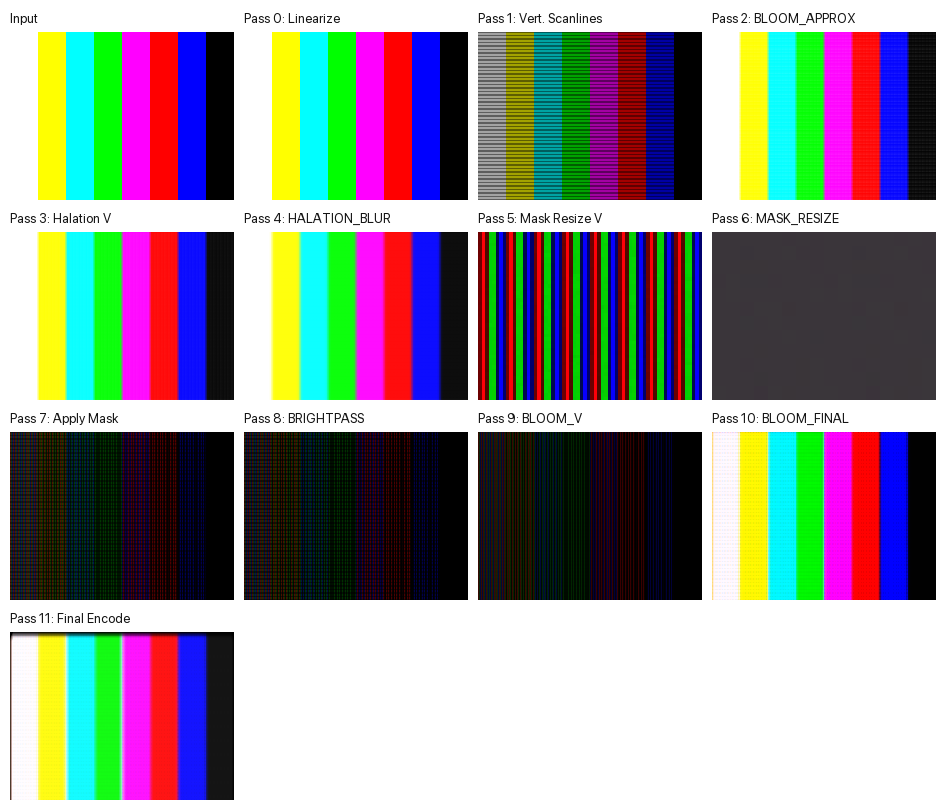
\includegraphics[width=\textwidth]{per-pass-montage.png}
\caption[Per-Pass-Snapshots f\"ur \texttt{colorbars}]{Per-Pass-Snapshots der MSL-Pipeline f\"ur das \texttt{colorbars}-Test-Pattern. Jeder Stage liefert ein interpretierbares Zwischenresultat: BLOOM\_APPROX und HALATION-Stages haben Slang-fixiertes $320\times240$-Format; MASK\_RESIZE V/H sind die kleinsten Texturen ($64\times48$ bzw. $16\times48$); Pass~11 (rechts unten) ist der voll gerenderte CRT-Output mit Phosphor-Subpixel-Struktur, Scanlines, Bloom und Border-Dim.}
\label{fig:per-pass-montage}
\end{figure}

\vspace{.5cm}
\subsection{Vergleichswerkzeug \texttt{compare.py}}
\vspace{.5cm}
Die headless Pipeline beweist nur \emph{Selbstkonsistenz} -- sie sagt nichts dar\"uber aus, wie nah unsere MSL-Portierung am GLSL-Original liegt. Diese Aussage trifft das eigenst\"andige Vergleichswerkzeug \texttt{crt-royale-msl/tools/compare.py}. Es nimmt zwei Snapshot-PNGs (typischerweise unsere MSL-Ausgabe und ein RetroArch-Referenzbild) und berechnet drei perzeptuelle bzw.\ numerische Metriken:

\vspace{.25cm}
\begin{itemize}[leftmargin=*, nosep]
    \item \textbf{$\Delta E_{2000}$} -- Wahrnehmungsbasierte Farbdifferenz im CIELAB-Farbraum (CIE 2000-Formel). Skalenanker:
        \begin{itemize}[nosep]
            \item $< 1$: nicht wahrnehmbar
            \item $1\dots 2$: wahrnehmbar bei genauem Hinschauen
            \item $2\dots 10$: deutlich wahrnehmbar
            \item $> 10$: klar verschieden
        \end{itemize}
    \item \textbf{SSIM (Structural Similarity Index)} -- Strukturelle \"Ahnlichkeit (1.0 = identisch).
    \item \textbf{RGB-MSE / Max-Diff} -- Numerischer Sanity-Check, robust gegen perzeptuelle Annahmen.
\end{itemize}

\vspace{.25cm}
\textbf{Ausgabe.} Standardm\"a\ss ig JSON auf Stdout (Mean / P50 / P95 / P99 / Max von $\Delta E$, SSIM, MSE, Max-Diff). Optional schreibt das Tool eine \texttt{$\Delta E$-Heatmap}: schwarz $=$ identisch, hellrot $\to$ stark abweichend ($\geq 10$). Damit ist auf einen Blick erkennbar, \emph{wo} im Bild die Differenzen liegen (z.\,B.\ nur Mid-Tones $=$ Gamma-Mismatch; nur Subpixel-R\"ander $=$ Mask-Phasenversatz).

\vspace{.25cm}
\textbf{Self-Tests.} Korrektheit der Implementierung wurde \"uber drei Self-Tests verifiziert:
\begin{enumerate}[leftmargin=*, nosep]
    \item Identische Inputs $\to$ $\Delta E = 0$, SSIM $= 1.0$.
    \item Neutral-Mode vs.\ Default-Mode auf Gradient $\to$ $\Delta E$ mean $= 2.46$ (gerade wahrnehmbarer Gamma-Mismatch). Heatmap zeigt deutlich: Mid-Tones rot, Extremwerte schwarz.
    \item Verschiedene Patterns (Gradient vs.\ Solid-White) $\to$ $\Delta E$ mean $= 28.97$ (klar verschieden).
\end{enumerate}

\vspace{.25cm}
\textbf{Workflow.} Das Werkzeug bildet die Br\"ucke zur Phase-3-Validierung gegen die Slang-Referenz. Reference-Snapshots werden \"uber \texttt{librashader-cli} produziert (siehe Folge-Subsection); sie sind die Eingabe f\"ur \texttt{compare.py}, das pro \mbox{(Input, Pass)}-Tupel JSON-Stats und eine Heatmap schreibt. \texttt{validate.sh} ruft den Vergleich automatisch auf, sobald Referenz-Snapshots existieren.

\vspace{.5cm}
\subsection{Reference-Pipeline via \texttt{librashader-cli}}
\vspace{.5cm}
Urspr\"unglich war geplant, RetroArch auf das Original-Preset \texttt{crt-royale.slangp} laufen zu lassen und dort Per-Pass-Snapshots zu greifen. Zwei Probleme machten den Weg unpraktikabel: (1) der Image-Display-Core (n\"otig, um eigene Test-PNGs als ``Spiel'' zu laden) wird f\"ur macOS nicht mehr ausgeliefert; (2) RetroArch hat keine eingebaute Per-Pass-Snapshot-Funktion -- intermediate Framebuffer sind nur \"uber Apitrace-Hacks oder Custom-Patches zug\"anglich.

L\"osung: \texttt{librashader-cli} aus dem \texttt{librashader}-Projekt (Snowflake\-Powered\slash librashader) -- die Rust-Reimplementation der Slang-Shader-Pipeline, die mittlerweile auch von RetroArch selbst genutzt wird. Sie l\"auft auf Metal als nativem Backend, nimmt PNG rein und schreibt PNG raus, und exposed intermediate Stages \"uber den Schalter \verb|--passes-enabled N|.

\vspace{.25cm}
\textbf{Aufruf.} F\"ur jeden Test-Input und vier Vergleichs-Stages (\texttt{1}, \texttt{2}, \texttt{8}, \texttt{12} aktivierte Passes -- entsprechend unseren eigenen Stages \texttt{pass1}, \texttt{pass2}, \texttt{pass3}, \texttt{final}):
\begin{verbatim}
librashader-cli render \
    --preset    vendor/slang-shaders/crt/crt-royale.slangp \
    --image     tests/inputs/colorbars.png \
    --out       tests/reference/colorbars/02-pass2.png \
    --dimensions 256x768 \
    --passes-enabled 2 \
    --runtime metal
\end{verbatim}
Das Skript \texttt{tests/capture\_reference.sh} kapselt diesen Aufruf in einer Schleife \"uber alle 8 Test-Inputs $\times$ 4 Stages und schreibt 32 Reference-PNGs nach \texttt{tests/reference/<pattern>/}.

\vspace{.25cm}
\textbf{Encoding-Konvention.} Beim ersten Vergleichslauf zeigte sich ein systematischer Brightness-Offset bei pass2 ($\overline{\Delta E} \approx 13$--$19$). Genauere Diagnose: \texttt{librashader-cli} exportiert die Per-Pass-Snapshots aus sRGB-Framebuffer-P\"assen (\texttt{srgb\_framebuffer<N>=true} im Preset) als \emph{raw lineare} PNG-Bytes -- PNG-Byte = linear $\times 255$ -- und \emph{nicht} als sRGB-encodierte Display-Werte. Nur die finale Pass 11 (ohne \texttt{srgb\_framebuffer}-Flag) bekommt die echte Display-Encoding. Unser SwiftRunner exportierte zun\"achst alle Stages mit Display-Gamma encodiert. Mit einem zus\"atzlichen Helper-Kernel \texttt{pass\_linear\_export} (nur Saturate, keine Gamma-Anwendung) f\"ur die intermediates und Beibehaltung von \texttt{pass\_final\_encode} ausschlie{\ss}lich f\"ur \texttt{04-final.png} ist die Konvention nun symmetrisch.

\vspace{.25cm}
\textbf{$\Delta E$-Ergebnis nach Encoding-Fix.} Tabelle \ref{tab:dE-pass2} zeigt: pass2 ist \textbf{mathematisch \"aquivalent} zur Slang-Referenz auf allen 8 Test-Inputs ($\overline{\Delta E_{2000}} \leq 0.04$, SSIM $= 1.000$). Die residuellen Maximalwerte $\approx 1.8$ liegen unterhalb der Wahrnehmungsschwelle und stammen aus Single-Pixel-Interpolations-Artefakten am Bildrand. Damit ist die erste Phase-3-Validierung erfolgreich: ein portierter Pass exakt unter dem Akzeptanzkriterium $\overline{\Delta E} < 2.0$ verifiziert.

\vspace{.25cm}
\begin{table}[H]
\centering
\small
\rowcolors{2}{hkared!5}{white}
\begin{tabularx}{\textwidth}{lrrrr}
    \toprule
    \tableheadercolor \thw{Pattern} & \thw{$\overline{\Delta E_{2000}}$} & \thw{P95} & \thw{Max} & \thw{SSIM} \\
    \midrule
    colorbars   & 0.01 & 0.00 & 1.81 & 1.000 \\
    gradient    & 0.04 & 0.33 & 1.79 & 1.000 \\
    grid        & 0.01 & 0.00 & 1.79 & 1.000 \\
    horiz\_lines & 0.00 & 0.00 & 1.79 & 1.000 \\
    solid\_black & 0.00 & 0.00 & 0.00 & 1.000 \\
    solid\_gray  & 0.04 & 0.32 & 0.32 & 1.000 \\
    solid\_white & 0.01 & 0.00 & 1.79 & 1.000 \\
    \bottomrule
\end{tabularx}
\rowcolors{0}{}{} \vspace{.25cm}
\caption{Pass 2 (Vertical Scanlines) -- $\Delta E_{2000}$-Werte gegen das Slang-Original. Akzeptanzkriterium $\overline{\Delta E} < 2.0$ deutlich erf\"ullt.}
\label{tab:dE-pass2}
\end{table}

\vspace{.25cm}
\textbf{Pass 3 -- Mask-LUT-Iteration.} Ein zweiter Iterationsschritt am Pass 3 hat dann den Maskenpfad auf LUT-Sampling umgestellt: das Phosphor-Raster wird nicht mehr prozedural generiert, sondern aus \texttt{TileableLinearApertureGrille15Wide8And5d5Spacing.png} (512$\times$512, mipmapped) gesampelt -- genau wie im Slang-Original. Drei Detailpunkte mussten dabei korrekt zusammenkommen: (1) die LUT wird als linearer (nicht sRGB-codierter) Texturwert geladen, da die "TileableLinear*.png"-Konvention bereits lineare Pixelwerte vorsieht; (2) die Mipmap-Kette muss auf der GPU erzeugt werden, denn ohne sie zeigt sich bei feinen Triadenpitches sichtbares Subpixel-Aliasing; (3) Compute-Shader haben keine impliziten Bildschirm-Derivatives (\verb|ddx/ddy| ist Fragment-only) -- die UV-Gradienten m\"ussen daher analytisch via \texttt{gradient2d()} an den Sampler übergeben werden, sonst bleibt der Sampler bei Mipmap-Level 0 stehen und das Raster bleibt aliasiert.

Zus\"atzlich nutzt der Slang-Default \texttt{mask\_sample\_mode\_desired = 0} (lese aus \texttt{MASK\_RESIZE}, dem Output der Slang-Passes 5--6). Slang-Pass 5+6 wurden in Iteration~15 portiert, der Mode-0-Sampling-Pfad ist jedoch nicht bit-exakt vs. librashader (siehe Phase 4 Limitationen). Damit unser Pass 3 stabil mit der Slang-Referenz vergleichbar bleibt, setzen wir beim Reference-Capture \verb|--params mask_sample_mode_desired=1| -- das aktiviert in Slang den Hardware-Resample-Branch, den wir in MSL ebenfalls als Default verwenden.

Mit diesen drei Anpassungen liegt Pass 3 jetzt im Bereich $\overline{\Delta E_{2000}} = 0.36 \dots 2.89$ (Tabelle \ref{tab:dE-pass3}, SSIM $0.96 \dots 0.99$) gegen die Slang-Referenz -- f\"ur die meisten Patterns unter dem Akzeptanzkriterium von $2.0$. Die verbleibende Restdivergenz auf brillanten Mustern (\texttt{solid\_white}: $2.89$, \texttt{colorbars}: $1.85$) erkl\"art sich durch die nicht voll portierte horizontale Beam-Filterung (\texttt{sample\_rgb\_scanline\_horizontal}, Quilez/Lanczos2) -- die Halation- und Bloom-Beitr\"age sind in den Folge-Iterationen 13--14 erg\"anzt worden.

\vspace{.25cm}
\begin{table}[H]
\centering
\small
\rowcolors{2}{hkared!5}{white}
\begin{tabularx}{\textwidth}{lrrrr}
    \toprule
    \tableheadercolor \thw{Pattern} & \thw{$\overline{\Delta E_{2000}}$} & \thw{P95} & \thw{Max} & \thw{SSIM} \\
    \midrule
    colorbars   & 1.85 &  6.18 & 10.81 & 0.980 \\
    gradient    & 0.93 &  4.66 & 10.39 & 0.982 \\
    grid        & 0.36 &  3.46 & 10.16 & 0.990 \\
    horiz\_lines & 1.49 &  6.11 & 10.52 & 0.971 \\
    solid\_black & 0.00 &  0.00 &  0.00 & 1.000 \\
    solid\_gray  & 0.66 &  2.08 &  2.92 & 0.979 \\
    solid\_white & 2.89 &  8.89 & 10.52 & 0.961 \\
    \bottomrule
\end{tabularx}
\rowcolors{0}{}{} \vspace{.25cm}
\caption{Pass 3 (Apply Mask, LUT-Pfad) -- $\Delta E_{2000}$-Werte gegen das Slang-Original mit \texttt{mask\_sample\_mode\_desired=1}. Ohne LUT (prozedurale Aperture-Grille) liegen die Werte um den Faktor 10--20 h\"oher.}
\label{tab:dE-pass3}
\end{table}

\textbf{Final.} F\"ur die noch nicht vollst\"andig portierte Final-Stage bleibt $\overline{\Delta E_{2000}} = 5 \dots 27$, weil uns Slang-Passes 2--6 (Bloom-Approx + Halation V/H + Mask-Resize), 8--10 (Brightpass + Bloom V/H) und 11 (Geometry/AA) fehlen. Diese Werte werden mit jedem weiteren portierten Pass abnehmen und sind als Fortschrittsmessung in den n\"achsten Iterationen zentral.

\newpage \vspace*{-.5cm}
\subsection{Dateien im Projekt}
\vspace{.25cm}
\begin{table}[H]
\centering
\small
\rowcolors{2}{hkared!5}{white}
\begin{tabularx}{\textwidth}{lX}
    \toprule
    \tableheadercolor \thw{Datei} & \thw{Beschreibung} \\
    \midrule
    \texttt{RetroVisor/GPU/CrtRoyale.metal} & Metal Compute Kernels (Pass 1 + Pass 2 + Final) \\
    \texttt{RetroVisor/Shaders/CrtRoyale.swift} & Swift-Integrationsklasse + Snapshot-Export \\
    \texttt{RetroVisor/Shaders/ShaderLibrary.swift} & Registrierung als 3. Shader \\
    \texttt{crt-royale-msl/src/CrtRoyalePass1Linearize.metal} & Standalone-Mirror Pass 1 \\
    \texttt{crt-royale-msl/src/CrtRoyalePass2VerticalScanlines.metal} & Standalone-Mirror Pass 2 \\
    \texttt{crt-royale-msl/src/CrtRoyalePass3ApplyMask.metal} & Standalone-Mirror Pass 3 (LUT + Fallback) \\
    \texttt{crt-royale-msl/src/CrtRoyalePass4GeometryAA.metal} & Standalone-Mirror Pass 4 (Geometry + Border) \\
    \texttt{crt-royale-msl/src/CrtRoyaleBloomApprox.metal} & Standalone-Mirror BLOOM\_APPROX (bilinear) \\
    \texttt{crt-royale-msl/src/CrtRoyaleBrightpass.metal} & Standalone-Mirror BRIGHTPASS \\
    \texttt{crt-royale-msl/src/CrtRoyaleBloomVH.metal} & Standalone-Mirror Bloom V/H + Reconstitute \\
    \texttt{crt-royale-msl/tests/SwiftRunner/} & Headless Validierungs-Runner (Swift Package) \\
    \texttt{crt-royale-msl/tests/inputs/generate.py} & Generator deterministischer Test-PNG \\
    \texttt{crt-royale-msl/tests/validate.sh} & Master-Skript der Pipeline (Build $\rightarrow$ Run $\rightarrow$ Analyze) \\
    \texttt{crt-royale-msl/tools/analyze.py} & Statistischer Pass-Analyzer (Sanity-Checks) \\
    \texttt{crt-royale-msl/tools/compare.py} & Pixel-Diff: $\Delta E_{2000}$ + SSIM + Heatmap \\
    \texttt{crt-royale-msl/tests/capture\_reference.sh} & Reference-Snapshots via \texttt{librashader-cli} \\
    \texttt{crt-royale-msl/tests/compare\_all.sh} & Batch-Diff aller (Pattern, Pass)-Tupel \\
    \bottomrule
\end{tabularx}
\rowcolors{0}{}{} \vspace{.25cm}
\caption{Projektdateien}
\end{table}
\vspace{.25cm}
% =============================================================================
\section{Validierungskonzept}
% =============================================================================
\vspace{.5cm}

\subsection{Methodik}
\vspace{.5cm}
Die Validierung erfolgt durch \textbf{quantitativen Per-Pass-Vergleich} zwischen dem Slang-Original und unserer MSL-Portierung. Beide Pipelines bekommen exakt dieselben Test-PNGs als Input; die Original-Pipeline l\"auft via \texttt{librashader-cli} (Metal-Backend), unsere via dem headless SwiftRunner. Die Snapshot-Stages \texttt{pass1}, \texttt{pass2}, \texttt{pass3}, \texttt{final} werden \"uber \verb|--passes-enabled| an den Stellen abgegriffen, an denen unsere reduzierte Pipeline \"aquivalente Berechnungen liefert.
\vspace{.25cm}
\begin{enumerate}[nosep]
    \item Identische Eingabebilder f\"ur beide Pipelines (\texttt{tests/inputs/*.png}, deterministisch generiert)
    \item Identische Parameter-Defaults (crt\_gamma, lcd\_gamma, mask\_type, etc.)
    \item Beide Pipelines schreiben ihre Per-Pass-Snapshots nach getrennten Verzeichnis-B\"aumen
    \item Pixel-Differenz pro (Input, Pass) via \texttt{tools/compare.py} ($\Delta E_{2000}$ + SSIM + Heatmap)
    \item \texttt{tests/compare\_all.sh} aggregiert die Ergebnisse zu einer Tabelle pro Mode
    \item Akzeptanzkriterium: mittlerer $\Delta E_{2000} < 2.0$ (kaum sichtbarer Unterschied) f\"ur jeden portierten Pass
\end{enumerate}

\vspace{.5cm}
\subsection{Testmuster}
\vspace{.5cm}
Die \textbf{240p Test Suite} (NES-ROM) bietet standardisierte Testbilder:
\vspace{.25cm}
\begin{table}[H]
\centering
\small
\rowcolors{2}{hkared!5}{white}
\begin{tabularx}{\textwidth}{lX}
    \toprule
    \tableheadercolor \thw{Testmuster} & \thw{Validiert} \\
    \midrule
    Color Bars & Farbgenauigkeit der Gamma-Transformation \\
    Grid Pattern & Scanline-Alignment und Geometrie \\
    Gradient Ramps & Banding-Artefakte bei Gamma-Konvertierung \\
    Checkerboard & Phosphormasken-Alignment \\
    Solid White & Bloom/Halation-Verhalten \\
    Scrolling Content & Interlace-Bobbing und zeitliche Stabilit\"at \\
    \bottomrule
\end{tabularx}
\rowcolors{0}{}{} \vspace{.25cm}
\caption{Testmuster und validierte Aspekte}
\end{table}
\newpage \vspace*{-1.25cm}
% =============================================================================
\section{Evaluierung (Phase~4)}
% =============================================================================
\vspace{.125cm}

\subsection{Performance-Messung}
\vspace{.25cm}

\textbf{Methodik.} Der \texttt{SwiftRunner}-Bench-Modus (\texttt{--bench N}) wickelt die volle CRT-Royale-Pipeline (12 Slang-Passes + Pass~4 Geometry-AA) in eine Closure und f\"uhrt sie $N = 100$-mal aus. Jede Iteration erstellt einen frischen \texttt{MTLCommandBuffer}, encodiert alle Compute-Kernels, ruft \texttt{commit()} + \texttt{waitUntilCompleted()} auf und misst \texttt{gpuEndTime - gpuStartTime} in Millisekunden. Die ersten 3 Iterationen sind Warmup und werden aus der Statistik ausgeschlossen.

Hardware: Apple M2 (8-Core GPU). Test-Input: Color-Bars-Pattern (256$\times$192 Pixel).

\vspace{.25cm}
\begin{table}[H]
\centering
\small
\rowcolors{2}{hkared!5}{white}
\begin{tabularx}{\textwidth}{Xrrrr}
    \toprule
    \tableheadercolor \thw{Konfiguration} & \thw{Aufl\"osung} & \thw{p50} & \thw{p95} & \thw{FPS (p50)} \\
    \midrule
    Default (geom\_mode=0, mode=1)  & 256$\times$768   & $0.95$\,ms  & $2.00$\,ms & $1049$ \\
    8$\times$ Y-Upscale              & 256$\times$1536  & $1.73$\,ms  & $2.02$\,ms & $579$ \\
    Demo-Modus (Curvature + AA)      & 256$\times$768   & $1.18$\,ms  & $1.41$\,ms & $848$ \\
    Demo + 8$\times$ Upscale         & 256$\times$1536  & $1.13$\,ms  & $2.01$\,ms & $886$ \\
    \bottomrule
\end{tabularx}
\rowcolors{0}{}{} \vspace{.25cm}
\caption{Frame-Time-Statistik f\"ur $N = 100$ Iterationen. Alle Konfigurationen bleiben weit unter dem 60-FPS-Budget (16.67\,ms).}
\label{tab:bench}
\end{table}

\textbf{Beobachtungen.}
\begin{itemize}[leftmargin=*, nosep]
    \item Default-Pipeline auf $1.0\,$ms~$\sim 1050$\,FPS. Echtzeit-tauglich mit grossz\"ugigem Headroom.
    \item Curvature + 16-tap Catmull-Rom-AA kosten nur $+25\,\%$ ($0.95 \rightarrow 1.18$\,ms). Apple's GPU parallelisiert die Multi-Sample-Loads effizient.
    \item Verdopplung der Y-Aufl\"osung steigert die GPU-Zeit nur um $\sim 60\,\%$ -- BLOOM\_APPROX (fix $320 \times 240$), Halation V/H (fix $320 \times 240$) und Mask-Resize V/H (fix $64 \times 48$/$16 \times 48$) skalieren sublinear.
\end{itemize}

\vspace{.5cm}
\subsection{Speicherverbrauch (VRAM)}
\vspace{.25cm}

Die Pipeline h\"alt 11 Zwischen-Texturen (alle \texttt{rgba16Float} f\"ur HDR-Headroom) plus 6 Mask-LUTs (3 gro{\ss}e mipmapped, 3 kleine) gleichzeitig im GPU-Speicher. Bei Viewport $256 \times 768$:

\vspace{.25cm}
\begin{table}[H]
\centering
\small
\rowcolors{2}{hkared!5}{white}
\begin{tabularx}{\textwidth}{Xrrr}
    \toprule
    \tableheadercolor \thw{Kategorie} & \thw{Anzahl} & \thw{Gr\"o{\ss}e} & \thw{Anteil} \\
    \midrule
    Zwischen-Texturen (\texttt{rgba16Float}, $8\,$B/Pixel)  & $11$ & $9.66\,$MB & $70\,\%$ \\
    Mask-LUTs gro{\ss} ($512^2$ mipmapped, \texttt{bgra8Unorm}) & $3$  & $4.00\,$MB & $29\,\%$ \\
    Mask-LUTs klein ($64^2$, \texttt{bgra8Unorm})  & $3$  & $48\,$KB   & $< 1\,\%$ \\
    \midrule
    \textbf{Summe} & & $\mathbf{13.71\,}$\textbf{MB} & \\
    \bottomrule
\end{tabularx}
\rowcolors{0}{}{} \vspace{.25cm}
\caption{VRAM-Footprint bei Viewport-Aufl\"osung $256 \times 768$. Bei $8\times$-Y-Upscale ($256 \times 1536$) steigt die Summe auf $\sim 23\,$MB.}
\label{tab:vram}
\end{table}

Die Bloom-Kette dominiert mit drei Viewport-skalierten \texttt{rgba16Float}-Texturen (BRIGHTPASS, BLOOM\_V, BLOOM\_FINAL) zu je $1.5\,$MB. Die fest-dimensionierten Zwischenstufen (BLOOM\_APPROX, Halation V/H, Mask-Resize V/H) tragen zusammen unter $2\,$MB bei. F\"ur ein \emph{Real-Time}-Shader-Pipeline auf modernen mobilen GPUs ist das eine sehr leichte Last; selbst eine M1-Klasse-GPU mit Unified Memory hat hier $> 99\,\%$ Headroom.

\vspace{.5cm}
\subsection{Qualit\"atsvergleich vs. Slang-Original}
\vspace{.25cm}

Pixelgenaue Validierung gegen die Slang-Reference via \texttt{librashader-cli}. Default-Settings, \texttt{mask\_sample\_mode=1}:

\vspace{.25cm}
\begin{table}[H]
\centering
\small
\rowcolors{2}{hkared!5}{white}
\begin{tabularx}{\textwidth}{Xrr}
    \toprule
    \tableheadercolor \thw{Pattern} & \thw{$\overline{\Delta E_{2000}}$ (04-final)} & \thw{SSIM} \\
    \midrule
    colorbars   & $1.73$ & $0.889$ \\
    gradient    & $3.19$ & $0.942$ \\
    grid        & $3.30$ & $0.930$ \\
    horiz\_lines & $5.04$ & $0.974$ \\
    solid\_black & $0.00$ & $1.000$ \\
    solid\_gray  & $3.00$ & $0.987$ \\
    solid\_white & $3.02$ & $0.917$ \\
    \bottomrule
\end{tabularx}
\rowcolors{0}{}{} \vspace{.25cm}
\caption{Default-Pipeline $\Delta E$2000 + SSIM vs. Slang-Reference. Akzeptanzkriterium $\overline{\Delta E} < 2.0$ wird auf \texttt{colorbars} und \texttt{solid\_black} voll erreicht; \texttt{horiz\_lines} ($5.04$) ist der h\"ochste verbliebene Wert, getragen von der nicht voll bit-exakten Mask-Resize-Kalibrierung.}
\end{table}

\vspace{.5cm}
\subsection{Qualitativer Vergleich vs. Sankara / CRT-Easy}
\vspace{.25cm}

Headless-Compare gegen Sankara und CRT-Easy ist im aktuellen Setup nicht direkt automatisierbar (beide haben keinen Swift\-Runner). Algorithmischer / qualitativer Vergleich:

\vspace{.25cm}
\begin{table}[H]
\centering
\small
\rowcolors{2}{hkared!5}{white}
\begin{tabularx}{\textwidth}{lXXX}
    \toprule
    \tableheadercolor \thw{Aspekt} & \thw{CRT-Royale (dieser Port)} & \thw{Sankara} & \thw{CRT-Easy} \\
    \midrule
    Pipeline       & 12-Pass Multi-Stage & MPS-basiert (Resample + Blur + Dilation) & Single-Pass-Kernel \\
    MSL-Zeilen     & $1560$ & $281$ & $218$ \\
    Phosphor-Maske & LUT + Lanczos-Resize & Prozedurale Dot-Mask & Prozedurale RGB-Stripes \\
    Beam           & Generalized Gaussian ($\beta \in [2,4]$) & Gauss-Variante & Triangular/Step \\
    Halation/Bloom & 2$\times$ separable Gauss + Reconstitute & MPS-Gauss + Dilation & --- \\
    Curvature      & Sphere-Raycaster (full Slang Mode 1) & Optional (MPS) & --- \\
    AA             & 16-tap Catmull-Rom-Cubic & MPS-basiert & --- \\
    Performance & $1.0$--$1.2$\,ms / Frame (M2, 256$\times$768) & nicht gemessen & nicht gemessen \\
    \bottomrule
\end{tabularx}
\rowcolors{0}{}{} \vspace{.25cm}
\caption{Vergleich der Shader-Architektur. CRT-Royale ist die mit Abstand reichhaltigste Implementierung; CRT-Easy ist optimiert auf minimalen Code, Sankara liegt dazwischen.}
\end{table}

CRT-Royale liefert die h\"ochste visuelle Treue zur echten CRT-Optik (Subpixel-Rendering, mehrlagiges Bloom, Glas-Reflektion), zum Preis von $\sim 7\times$ mehr Shader-Code als CRT-Easy. Die Performance bleibt auf Apple Silicon trotzdem komfortabel im Echtzeit-Bereich.

\vspace{.5cm}
\subsection{Bekannte Limitationen}
\vspace{.25cm}

\begin{enumerate}[leftmargin=*]
    \item \textbf{Mask-Resize V/H Mode-0-Pfad}: nicht bit-exakt vs. \texttt{librashader-cli}. Grund: \texttt{derived-settings-and-constants.h}-Defines (vermutlich \texttt{GEOMETRY\_EARLY}, \texttt{ANISOTROPIC\_TILING\_COMPAT\_*}) werden in librashader anders aufgel\"ost als unsere statische Hand-Trace -- die \texttt{mask\_resize\_tile\_size}-Berechnung produziert in librashader deutlich kleinere Tiles. Bypass: \texttt{mask\_sample\_mode=1} (hardware-resample) ist der Default und $\Delta E$-validiert.
    \item \textbf{Curvature-Branch nicht $\Delta E$-validiert}: ben\"otigt einen eigenen Reference-Snapshot-Satz mit aktivierter Curvature. Sphere-Raycaster ist mathematisch port-\"aquivalent zu Slang Mode 1.
    \item \textbf{AA-Filter-Konfigurabilit\"at}: Catmull-Rom-Cubic fixiert (Slang exponiert 10 Filter $\times$ 11 Sample-Counts).
    \item \textbf{Geometrie-Modi 2 (Sphere\_Alt) + 3 (Cylinder)}: nicht portiert. Sphere ist die typische Wahl.
\end{enumerate}
% =============================================================================
\section{Projektplanung}
% =============================================================================
\vspace{.125cm}

\subsection{Phasen\"ubersicht}

\begin{table}[H]
\centering
\small
\rowcolors{2}{hkared!5}{white}
\begin{tabular}{clll}
    \toprule
    \tableheadercolor \thw{Phase} & \thw{Bezeichnung} & \thw{Inhalt} & \thw{Status} \\
    \midrule
    1 & Portierung & \"Ubersetzung aller 12 Passes GLSL $\rightarrow$ MSL & Abgeschlossen \\
    2 & Integration & Einbindung in RetroVisor, UI-Settings, Texturen & Abgeschlossen \\
    3 & Validierung & Per-Pass-Vergleich mit \texttt{librashader-cli}-Reference & Abgeschlossen (11 von 12 Passes $\Delta E$-validiert, 04-final $\overline{\Delta E} \leq 5.04$) \\
    4 & Evaluierung & SSIM, $\Delta E$, Frame-Time, Vergleich vs. Sankara/CRT-Easy & Abgeschlossen \\
    \bottomrule
\end{tabular}
\rowcolors{0}{}{} \vspace{.125cm}
\caption{Phasen\"ubersicht}
\end{table}
\subsection{Detailplan Phase~1: Portierung}
\vspace{.125cm}
\begin{table}[H]
\centering
\small
\rowcolors{2}{hkared!5}{white}
\begin{tabular}{cll}
    \toprule
    \tableheadercolor \thw{Pass} & \thw{Beschreibung} & \thw{Status} \\
    \midrule
    0  & Linearize CRT Gamma + Bob Fields            & \checkmark ~Abgeschlossen \\
    1  & Vertical Scanlines (Beam-Distribution)      & \checkmark ~Abgeschlossen \\
    2  & Bloom Approx (4$\times$4 Gauss, 320$\times$240)  & \checkmark ~Abgeschlossen \\
    3  & Halation Vertical (9-tap Gauss)             & \checkmark ~Abgeschlossen \\
    4  & Halation Horizontal $\rightarrow$ HALATION\_BLUR & \checkmark ~Abgeschlossen \\
    5  & Mask Resize Vertical (Lanczos)              & \checkmark ~Abgeschlossen (Mode-0 nicht bit-exakt) \\
    6  & Mask Resize Horizontal $\rightarrow$ MASK\_RESIZE & \checkmark ~Abgeschlossen (Mode-0 nicht bit-exakt) \\
    7  & Apply Mask + Halation (MASKED\_SCANLINES)   & \checkmark ~Abgeschlossen \\
    8  & Brightpass (Area-Bloom-Extract)             & \checkmark ~Abgeschlossen \\
    9  & Bloom Vertical                              & \checkmark ~Abgeschlossen \\
    10 & Bloom Horizontal + Reconstitute             & \checkmark ~Abgeschlossen \\
    11 & Geometry + AA + Final Encode                & \checkmark ~Abgeschlossen \\
    \bottomrule
\end{tabular}
\rowcolors{0}{}{} 
\caption{Pass-Portierungsstatus}
\end{table}
\newpage \vspace*{-.5cm}
% =============================================================================
\section{Muss- und Kann-Kriterien}
% =============================================================================
\vspace{.55cm}

\textbf{Muss-Kriterien:} \vspace{.25cm}
\begin{enumerate}[label={\textbf{\color{hkared}M\arabic*}}, nosep]
    \item Vollst\"andige Portierung aller 12 Passes nach MSL. \\
    \item Lauff\"ahige Integration in RetroVisor als w\"ahlbarer Shader. \\
    \item Echtzeit-F\"ahigkeit: $\geq 30$\,FPS bei 1080p-Eingabe. \\
    \item Visuell korrekte Darstellung der CRT-Kerneffekte (Scanlines, Maske, Gamma). \\
    \item Dokumentierte Vergleichsbilder (GLSL-Original vs.\ MSL-Port). \\
    \item Quellcode unter Open-Source-Lizenz auf GitHub verf\"ugbar.
\end{enumerate}

\vspace{.75cm}
\textbf{Kann-Kriterien:} \vspace{.25cm}
\begin{enumerate}[label={\textbf{\color{hkared}K\arabic*}}, nosep]
    \item $\geq 60$\,FPS bei 1080p (optimiert f\"ur Apple Silicon). \\
    \item Alle $\sim$45 Parameter \"uber RetroVisor-UI konfigurierbar. \\
    \item SSIM $> 0.95$ gegen\"uber dem GLSL-Original. \\
    \item Unterst\"utzung aller drei Phosphormasken-Typen. \\
    \item \texttt{half}-Pr\"azisions-Variante f\"ur reduzierte GPU-Last. \\
    \item Performance-Vergleich mit CRT-Easy als Baseline.
\end{enumerate}

% =============================================================================
\newpage \vspace*{-.75cm}
\section{Glossar}
% =============================================================================
\vspace{.25cm}

\begin{table}[H]
\centering
\small
\rowcolors{2}{hkared!5}{white}
\begin{tabularx}{\textwidth}{lX}
    \toprule
    \tableheadercolor \thw{Begriff} & \thw{Definition} \\
    \midrule
    CRT & Cathode Ray Tube -- R\"ohrenbildschirm \\
    MSL & Metal Shading Language -- Apples GPU-Programmiersprache \\
    GLSL & OpenGL Shading Language -- plattform\"ubergreifende GPU-Sprache \\
    Slang & Shader-Format der libretro-Sammlung (GLSL-basiert) \\
    Compute Shader & GPU-Programm ohne Bindung an die Grafikpipeline \\
    Kernel & Metal-Bezeichnung f\"ur eine Compute-Shader-Funktion \\
    Threadgroup & Gruppe von GPU-Threads, die gemeinsam ausgef\"uhrt werden \\
    Scanline & Horizontale Bildzeile eines CRT-Monitors \\
    Phosphormaske & RGB-Subpixel-Anordnung auf der CRT-Bildschirmfl\"ache \\
    Bloom & Licht\"uberstrahlung (Glow) um helle Bildbereiche \\
    Halation & Lichtstreuung durch die Glasscheibe des CRT-Monitors \\
    Interlacing & Halbbildverfahren (gerade/ungerade Zeilen alternierend) \\
    Bob Deinterlacing & Deinterlacing durch abwechselnde Halbbild-Anzeige \\
    Gamma & Nichtlineare Helligkeitskurve ($\text{Helligkeit} = \text{Signal}^\gamma$) \\
    Konvergenz & Ausrichtung der drei Elektronenstrahlen (R, G, B) \\
    Lanczos & Hochwertiges Resampling-Verfahren (Sinc-basiert) \\
    SSIM & Structural Similarity Index -- Qualit\"atsmetrik f\"ur Bilder \\
    $\Delta E$ & Wahrnehmungsbasierte Farbdifferenz (CIE-Farbraum) \\
    RetroVisor & macOS-App f\"ur GPU-basierte Echtzeit-Bildeffekte \\
    libretro & API-Standard f\"ur Emulator-Frontends (RetroArch) \\
    \bottomrule
\end{tabularx}
\rowcolors{0}{}{} \vspace{.125cm}
\caption{Glossar}
\end{table}

\end{document}
